\documentclass[aspectratio=169]{beamer}

%---------------------------
%       Beamer Cheat Sheet
%---------------------------
% https://www.cpt.univ-mrs.fr/~masson/latex/Beamer-appearance-cheat-sheet.pdf

%---------------------------
%       Set Theme and Colors
%---------------------------

\usetheme[width=.1\paperwidth]{Hannover}
% \setbeamertemplate{sidebar canvas right}[vertical shading][top=red,bottom=blue]

\definecolor{QESblue}{HTML}{8AD2ED}
\definecolor{QESdarkblue}{HTML}{187ca2}
\definecolor{QESlightblue}{HTML}{c4e8f6}

\setbeamercolor{sidebar}{bg=QESlightblue}
\setbeamercolor{titlelike}{fg=QESdarkblue}

\setbeamercolor{palette sidebar secondary}{fg=QESdarkblue}
\setbeamercolor{title in sidebar}{fg=QESdarkblue}
\setbeamercolor{author in sidebar}{fg=QESdarkblue}

\addtobeamertemplate{sidebar left}{}{\vfill \hspace{.006\paperwidth} 
\includegraphics[width=.08\paperwidth]{../../../logo.png} \vspace{.006\paperwidth} } 
% \addtobeamertemplate{sidebar left}{}{\vfill \hspace{.00001\paperwidth} 
\includegraphics[width=.093\paperwidth]{../../figures/qes-qr.png} \vspace{.003\paperwidth} } 

%---------------------------
%       No navigation symbols
%---------------------------
\setbeamertemplate{navigation symbols}{}

%---------------------------
%       Set Fonts
%---------------------------
\usepackage{helvet}
\renewcommand{\familydefault}{\sfdefault}
\usepackage{sansmathfonts}
\usepackage{upgreek}

\setbeamerfont{frametitle}{series=\bfseries, size=\Large}
\setbeamerfont{title in sidebar}{series=\bfseries, size=\small}
\setbeamertemplate{caption}{\it\raggedright\insertcaption\par}

%---------------------------
%       Math font packages
%---------------------------
\usepackage{dsfont, amsmath, amsthm, mathtools}
\usepackage{bbm, bm}
\usepackage[T1]{fontenc}
\usepackage[version=3]{mhchem}

%---------------------------
%       Figure packages
%---------------------------
\usepackage{graphicx}
\graphicspath{{../../figures}}

\usepackage{epstopdf}
\usepackage{color}

\setbeamerfont{caption}{size=\footnotesize}

\usepackage{subfigure}

%---------------------------
%       Manual placement packages
%---------------------------
\usepackage{tikz}
\usetikzlibrary{calc}

%---------------------------
%       Local Macros
%---------------------------

\newcommand{\manualpic}[4]{
    % inputs {filename}{figure options}{x offset}{y offset}
    \tikz[remember picture, overlay] \node[anchor=center] at ($(current page.center)+(#3,#4)$) {\includegraphics[#2]{#1}};
}

\newcommand{\manualtext}[3]{
    % inputs {text}{x offset}{y offset}
    \tikz[remember picture, overlay] \node[anchor=center] at ($(current page.center)+(#2,#3)$) {#1};
}

\newcommand{\manualtextleft}[3]{
    % inputs {text}{x offset}{y offset}
    \tikz[remember picture, overlay] \node[anchor=west] at ($(current page.center)+(#2,#3)$) {#1};
}

\newcommand{\manualtextright}[3]{
    % inputs {text}{x offset}{y offset}
    \tikz[remember picture, overlay] \node[anchor=east] at ($(current page.center)+(#2,#3)$) {#1};
}

\newcommand{\slidereference}[1]{
    \manualtextleft{\tiny #1}{-0.47\linewidth}{-0.47\textheight}
}

\newcommand{\dv}[2]{\frac{\mathrm{d}#1}{\mathrm{d}#2}}

\title{Future Climate}
\author{Timescales}

\begin{document}

% (Branson) Friday March 10th - Lecture 45 – Future Climate 2: Timescales. 
% Introduce the idea that the climate system has momentum and inertia.
% What changes are we already committed to, and what are their timescales?
% What does recovery look like?

\begin{frame}{Future Climate\\Timescales \& Recovery}
    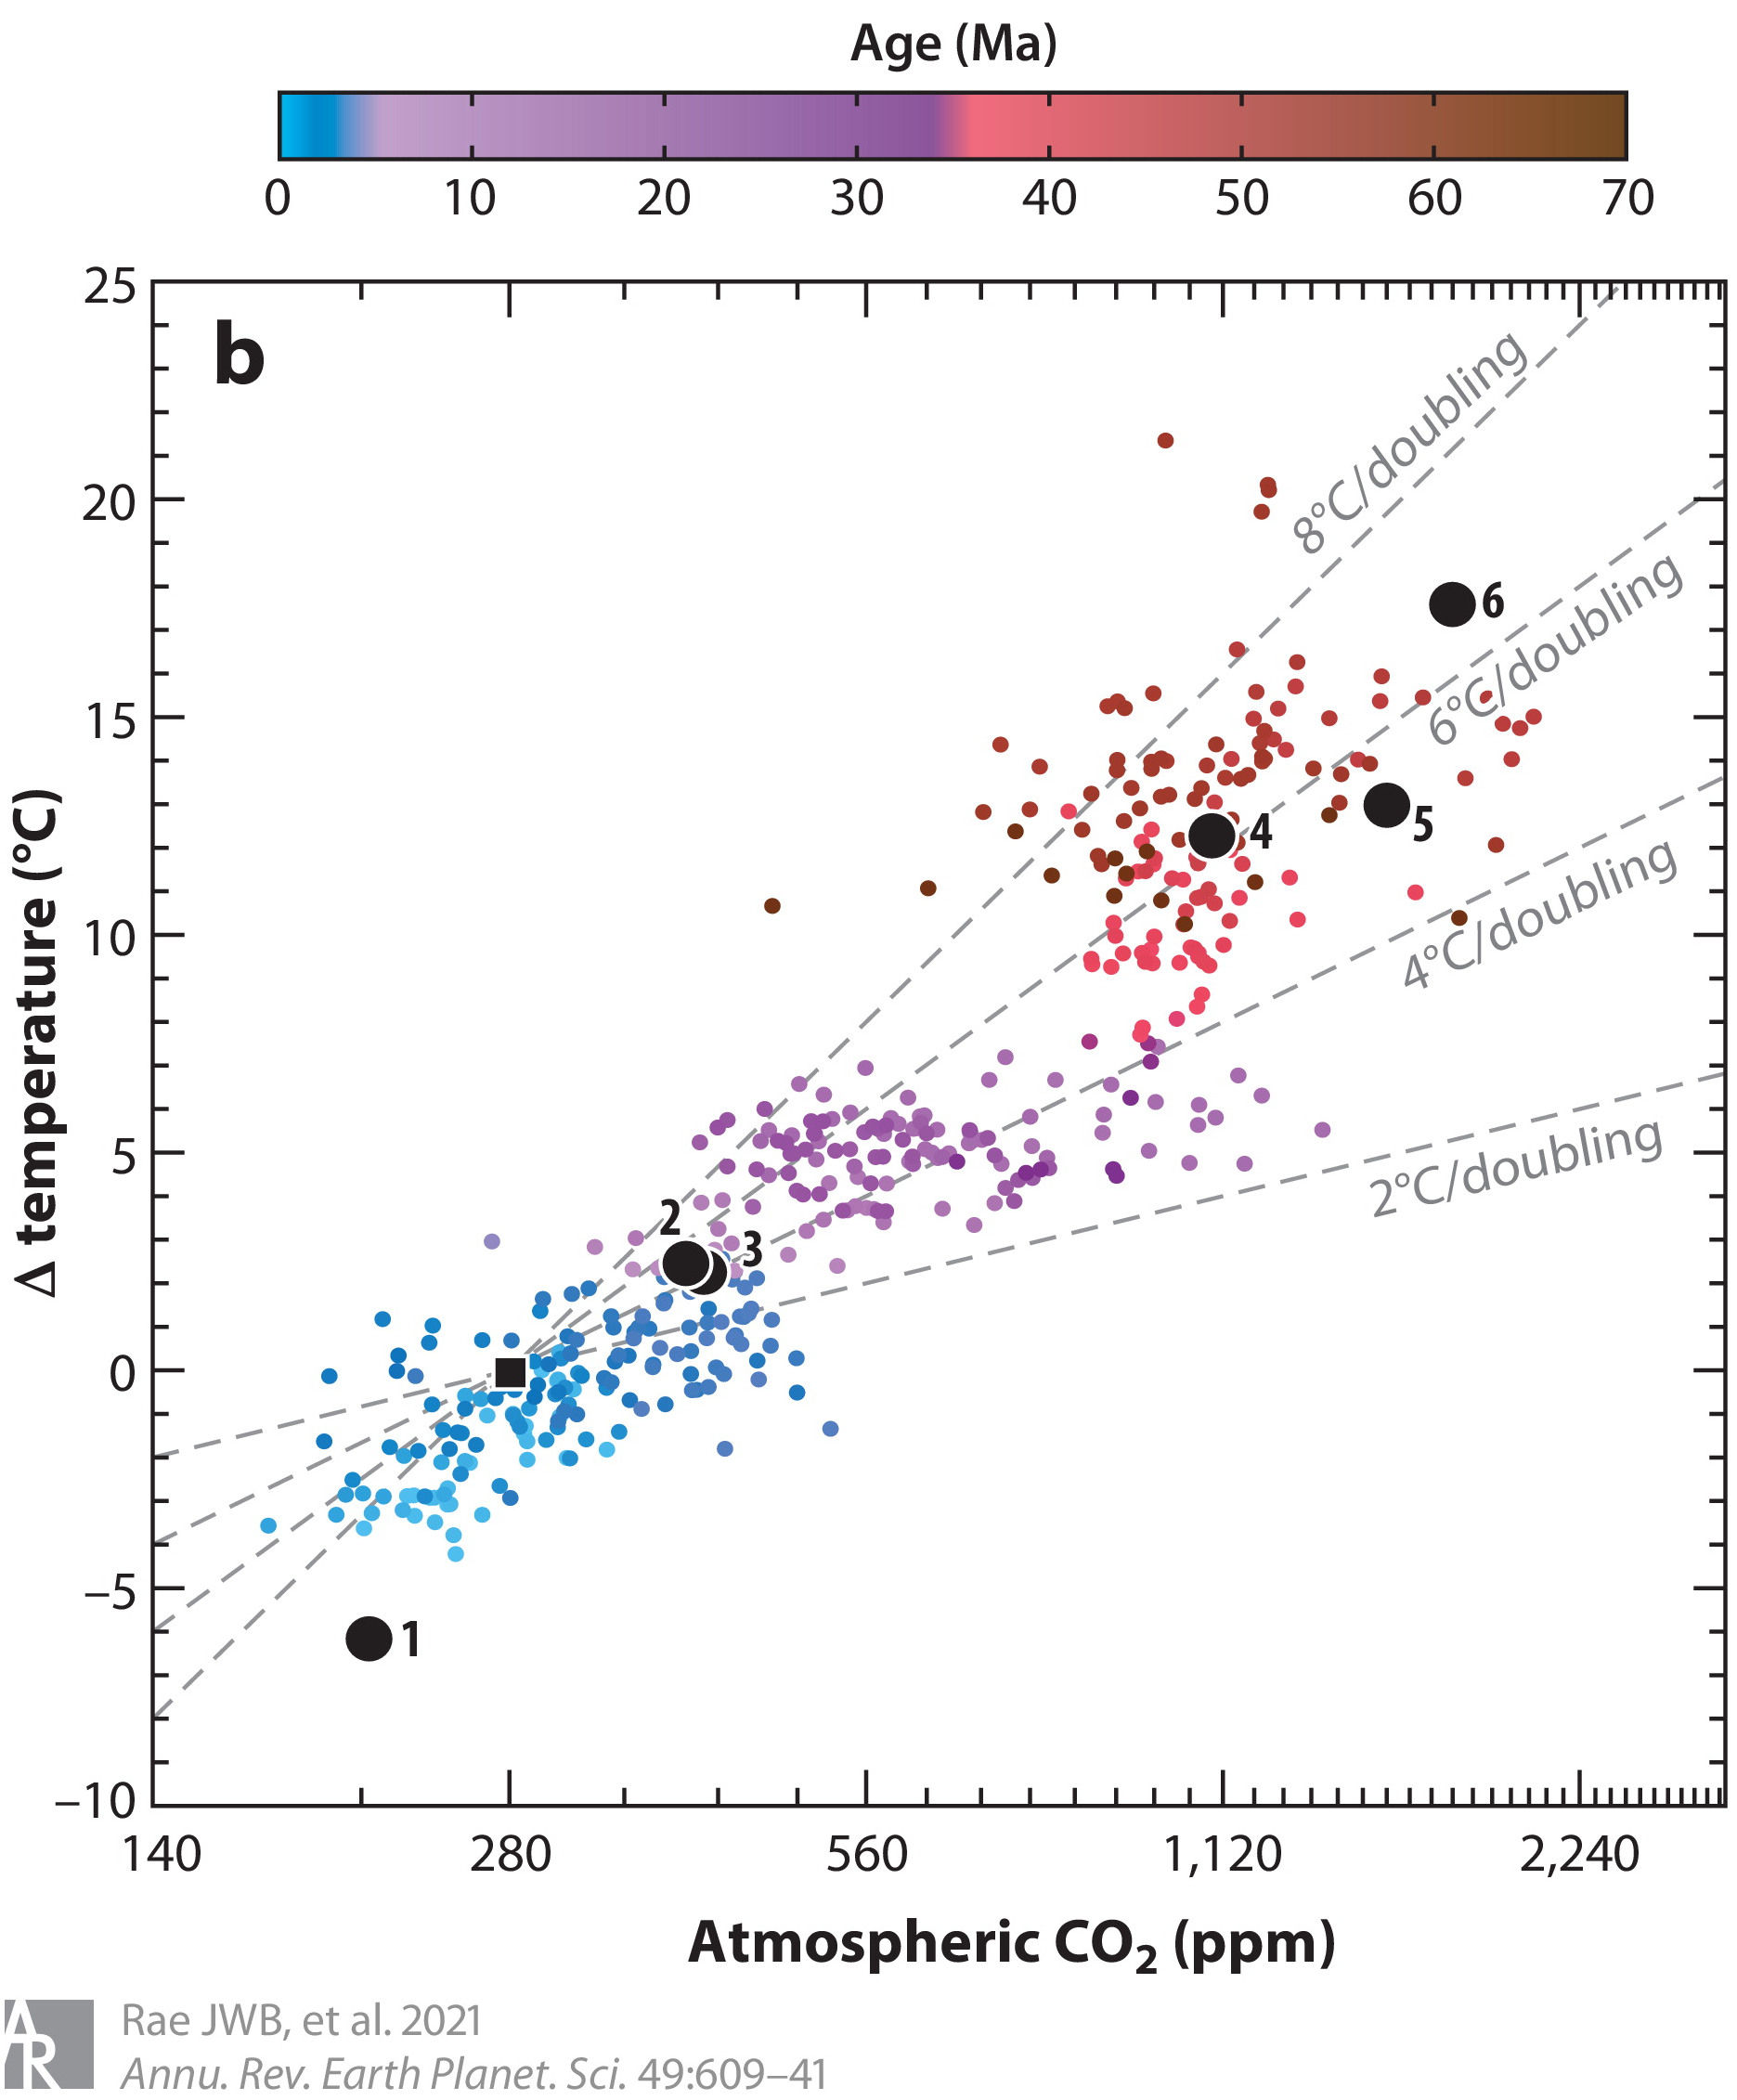
\includegraphics[width=\linewidth, totalheight=0.8\textheight, keepaspectratio]{future-palaeo-sensitivity.jpeg}
\end{frame}

\begin{frame}{Aims}

    \begin{enumerate}
        \item There is \textbf{considerable uncertainty} in climate models.
        \item The Climate System has \textbf{Momentum} and \textbf{Inertia}.
        \item \textbf{Climate Sensitivity} is a crucial unknown.
        \item Uncetainties arise from pushing the climate into an \textbf{unseen state}.
        \item \textbf{Past Climates} offer constraints on sensitivity\dots
        \item \dots and insights into \textbf{recovery}.
        \item \textbf{Climate Action is Urgent!}
    \end{enumerate}

\end{frame}

\section{(Un)certainty}

\begin{frame}{Uncertainty}
    % weather vs. climate - specific predictions hard; average predictions more certain
    \centering
    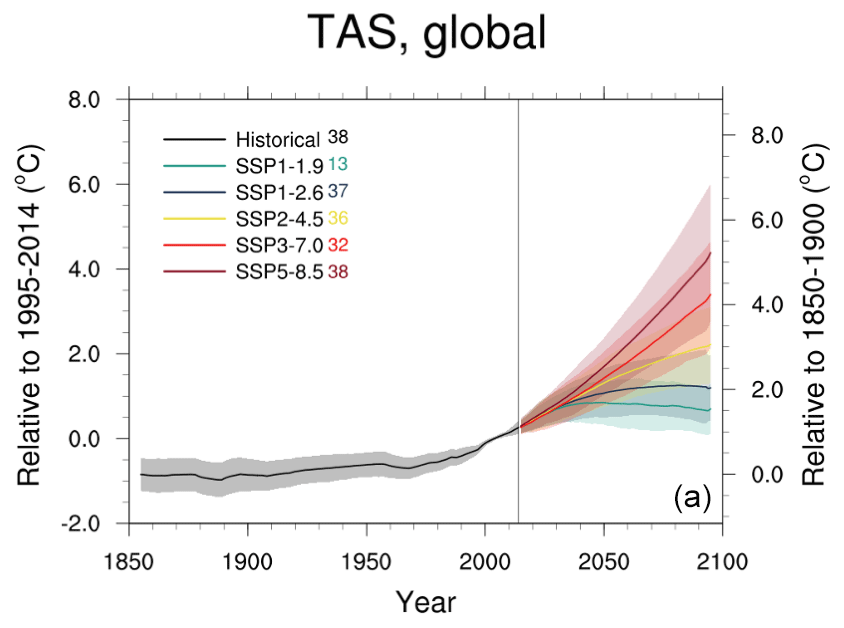
\includegraphics[width=\linewidth, totalheight=0.82\textheight, keepaspectratio]{future-Tabaldi-CMIP6-TAS.png}
    \slidereference{Tabaldi et al., 2021}
\end{frame}

\begin{frame}<handout:0>{Uncertainty}
    % weather vs. climate - specific predictions hard; average predictions more certain
    \centering
    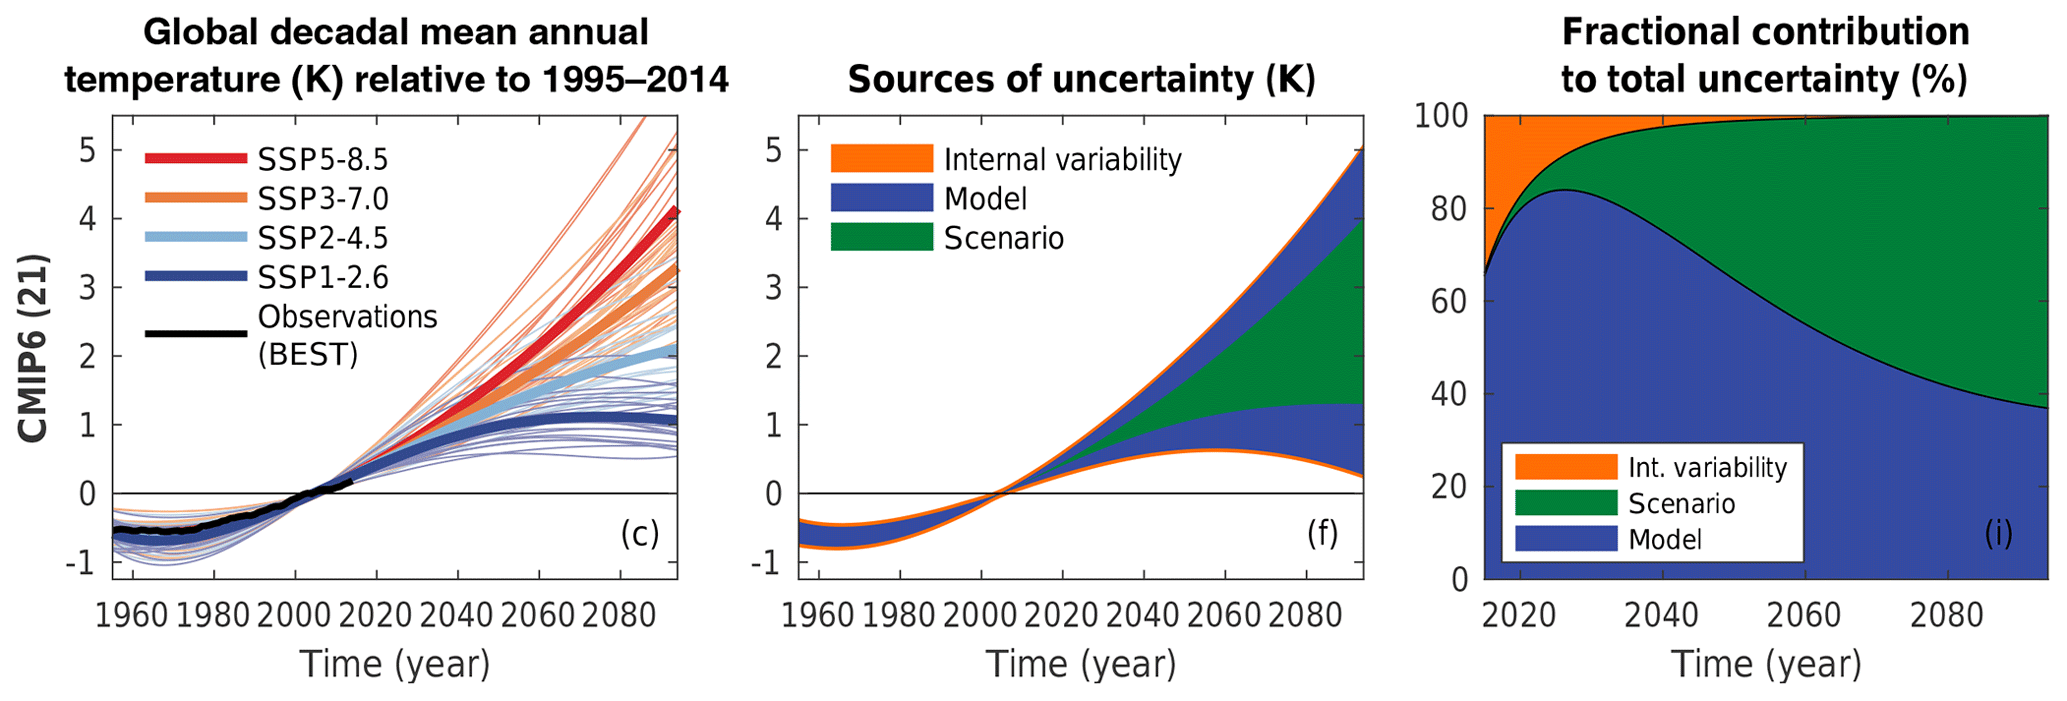
\includegraphics[width=\linewidth, totalheight=0.82\textheight, keepaspectratio]{future-Lehner-uncertainty.png}
    \slidereference{Lehner et al., 2020}
\end{frame}

\begin{frame}{Uncertainty: Scenario}
    % weather vs. climate - specific predictions hard; average predictions more certain
    \centering
    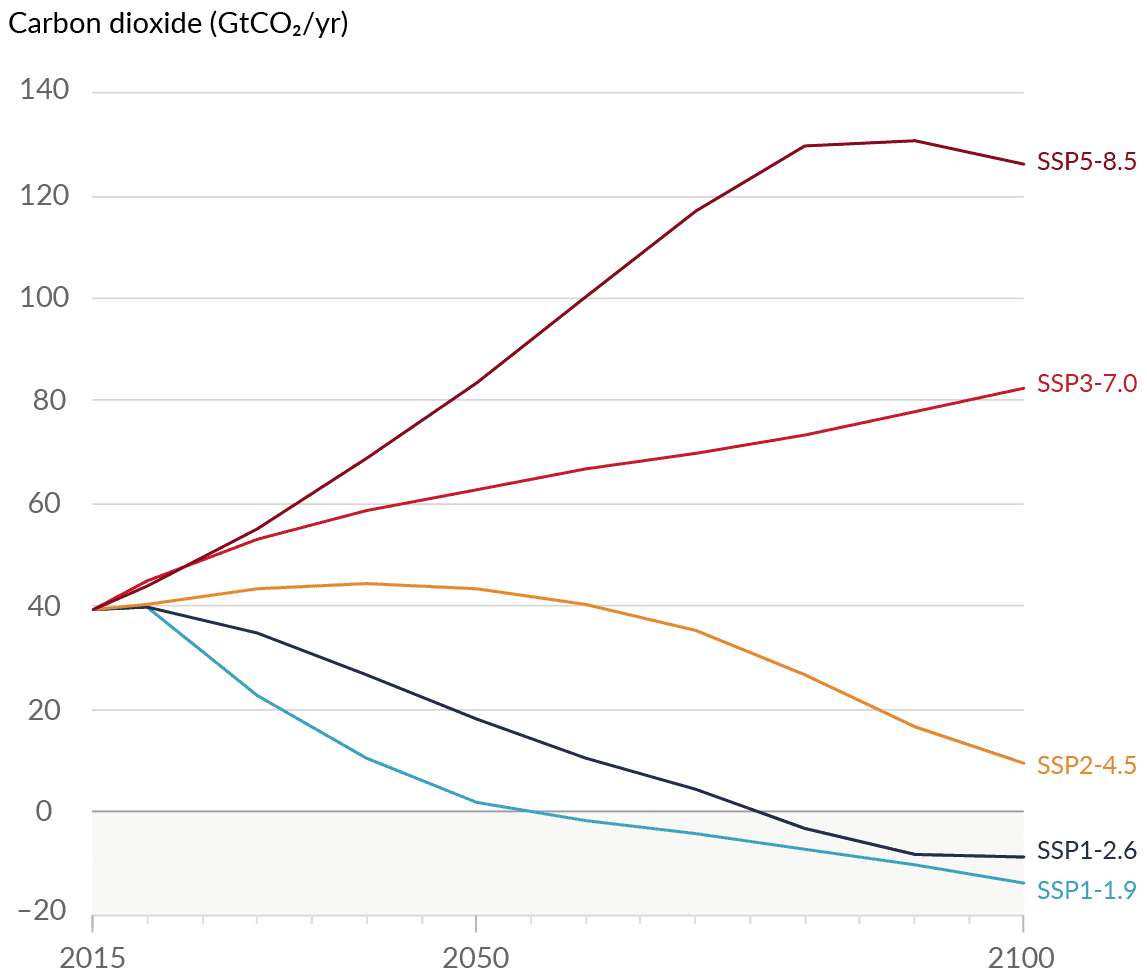
\includegraphics[width=\linewidth, totalheight=0.82\textheight, keepaspectratio]{future-emission-scenarios.png}
    \slidereference{IPCC AR6, SPM}
\end{frame}

\begin{frame}{Uncertainty}
    % weather vs. climate - specific predictions hard; average predictions more certain
    \centering
    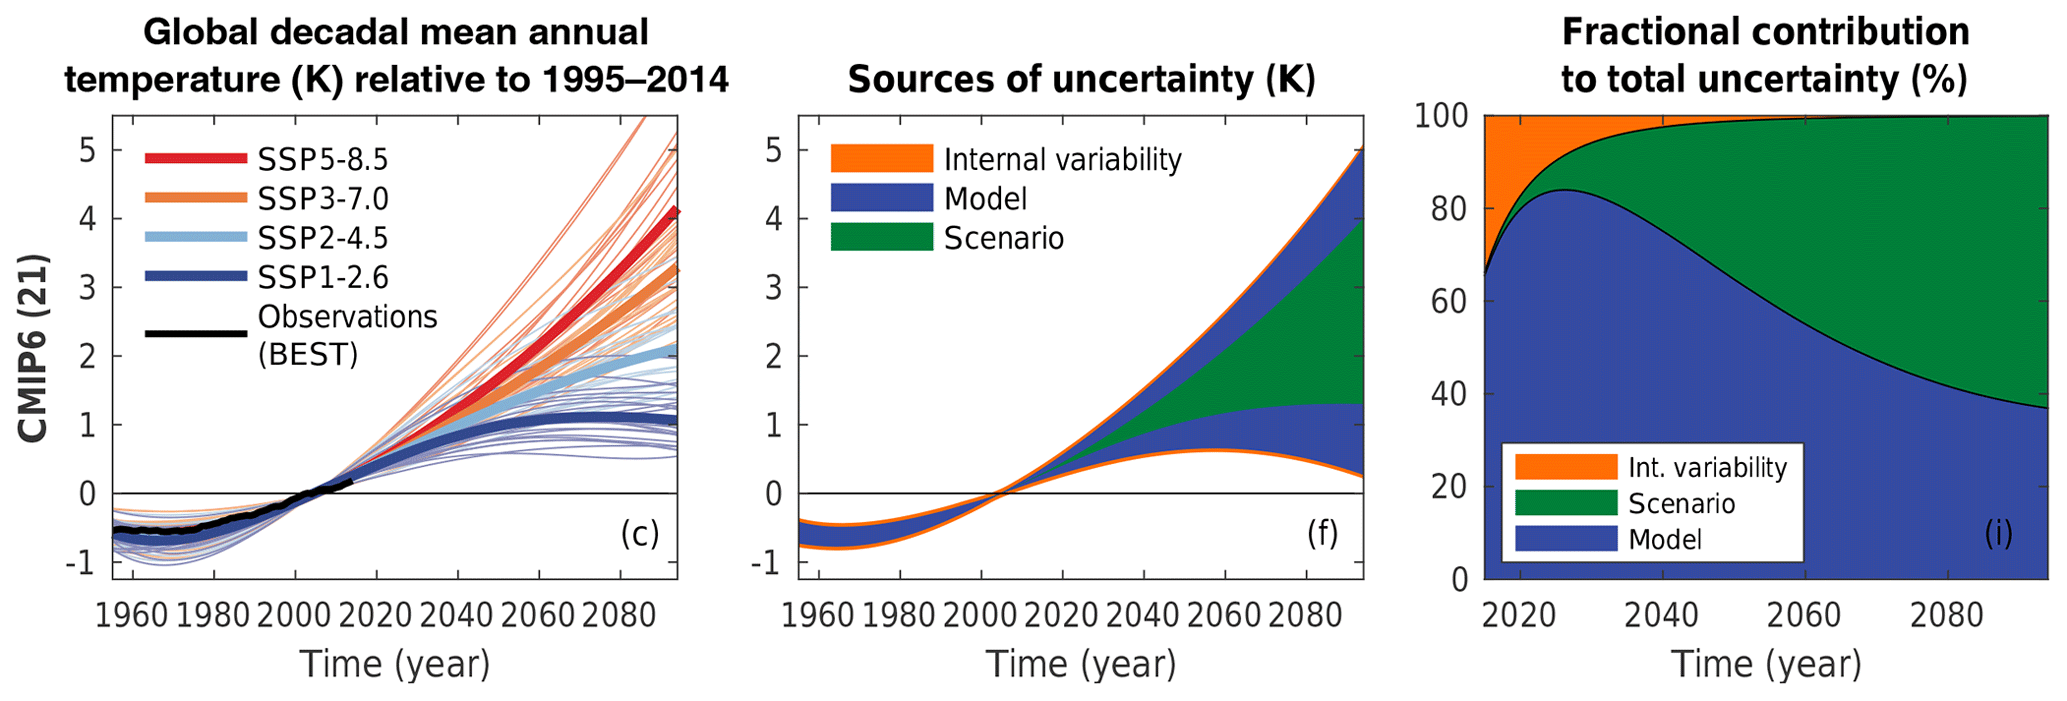
\includegraphics[width=\linewidth, totalheight=0.82\textheight, keepaspectratio]{future-Lehner-uncertainty.png}

    \onslide<2|handout:1>{$\sim$ 40 \% of uncertainty comes from model choice!}

    \slidereference{Lehner et al., 2020}
\end{frame}

\section{Future Climate}

\begin{frame}{Certainty}
    \centering
    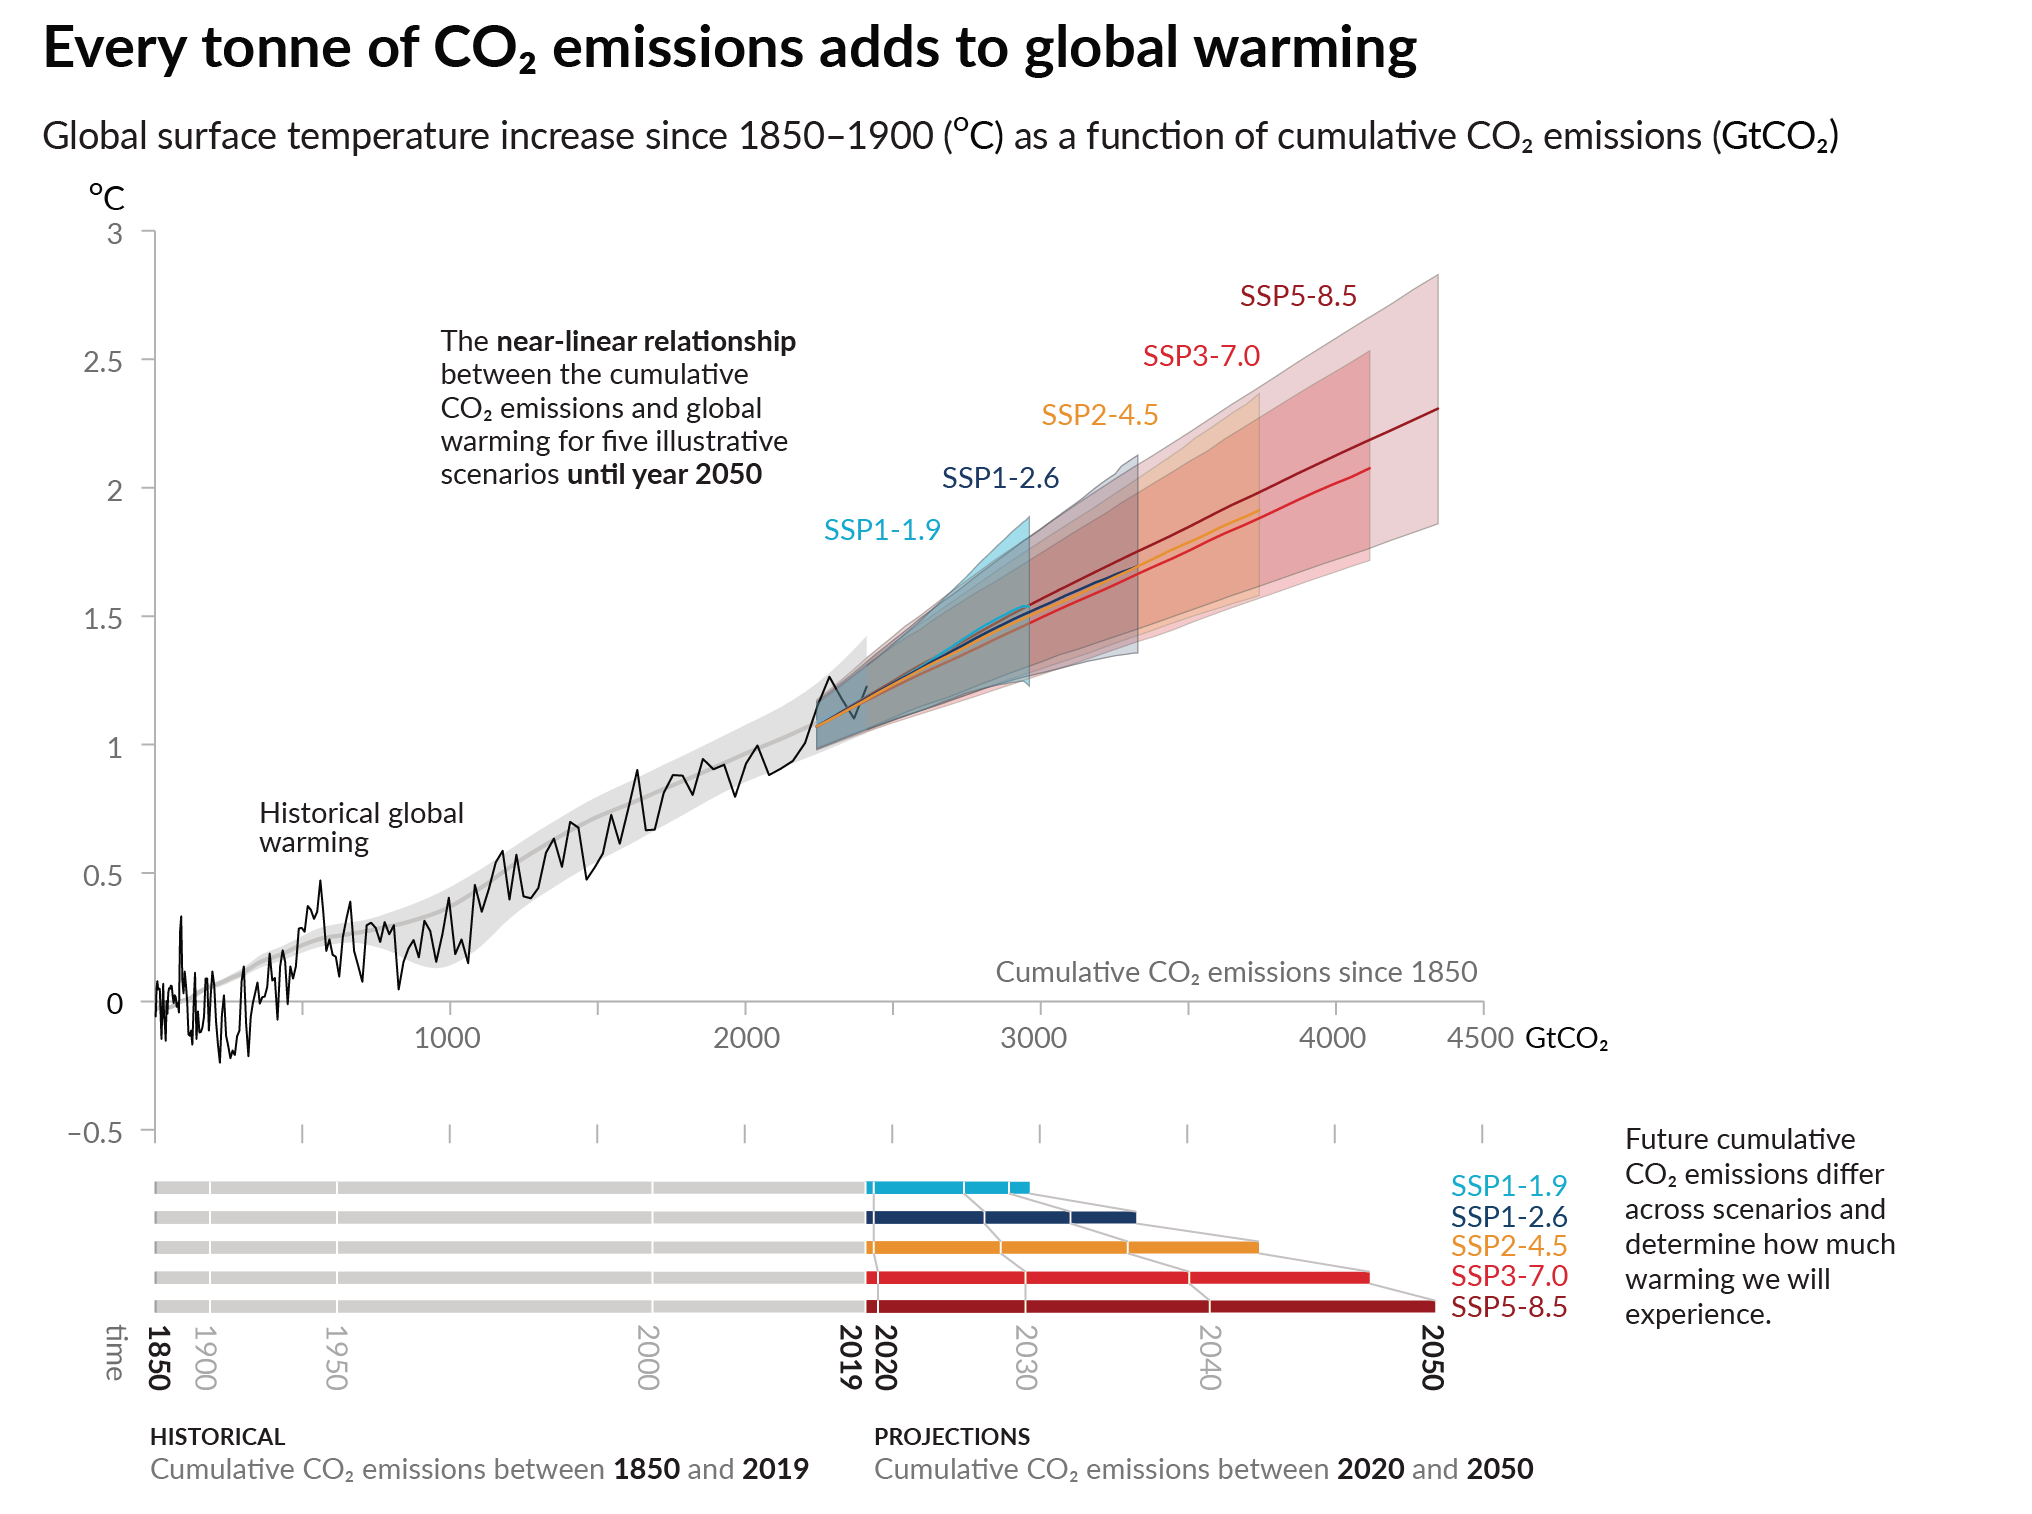
\includegraphics[width=\linewidth, totalheight=0.82\textheight, keepaspectratio]{future-SPM_Figure_10.png}
    \slidereference{IPCC AR6, SPM}
\end{frame}

\begin{frame}{Feedbacks}
    \centering
    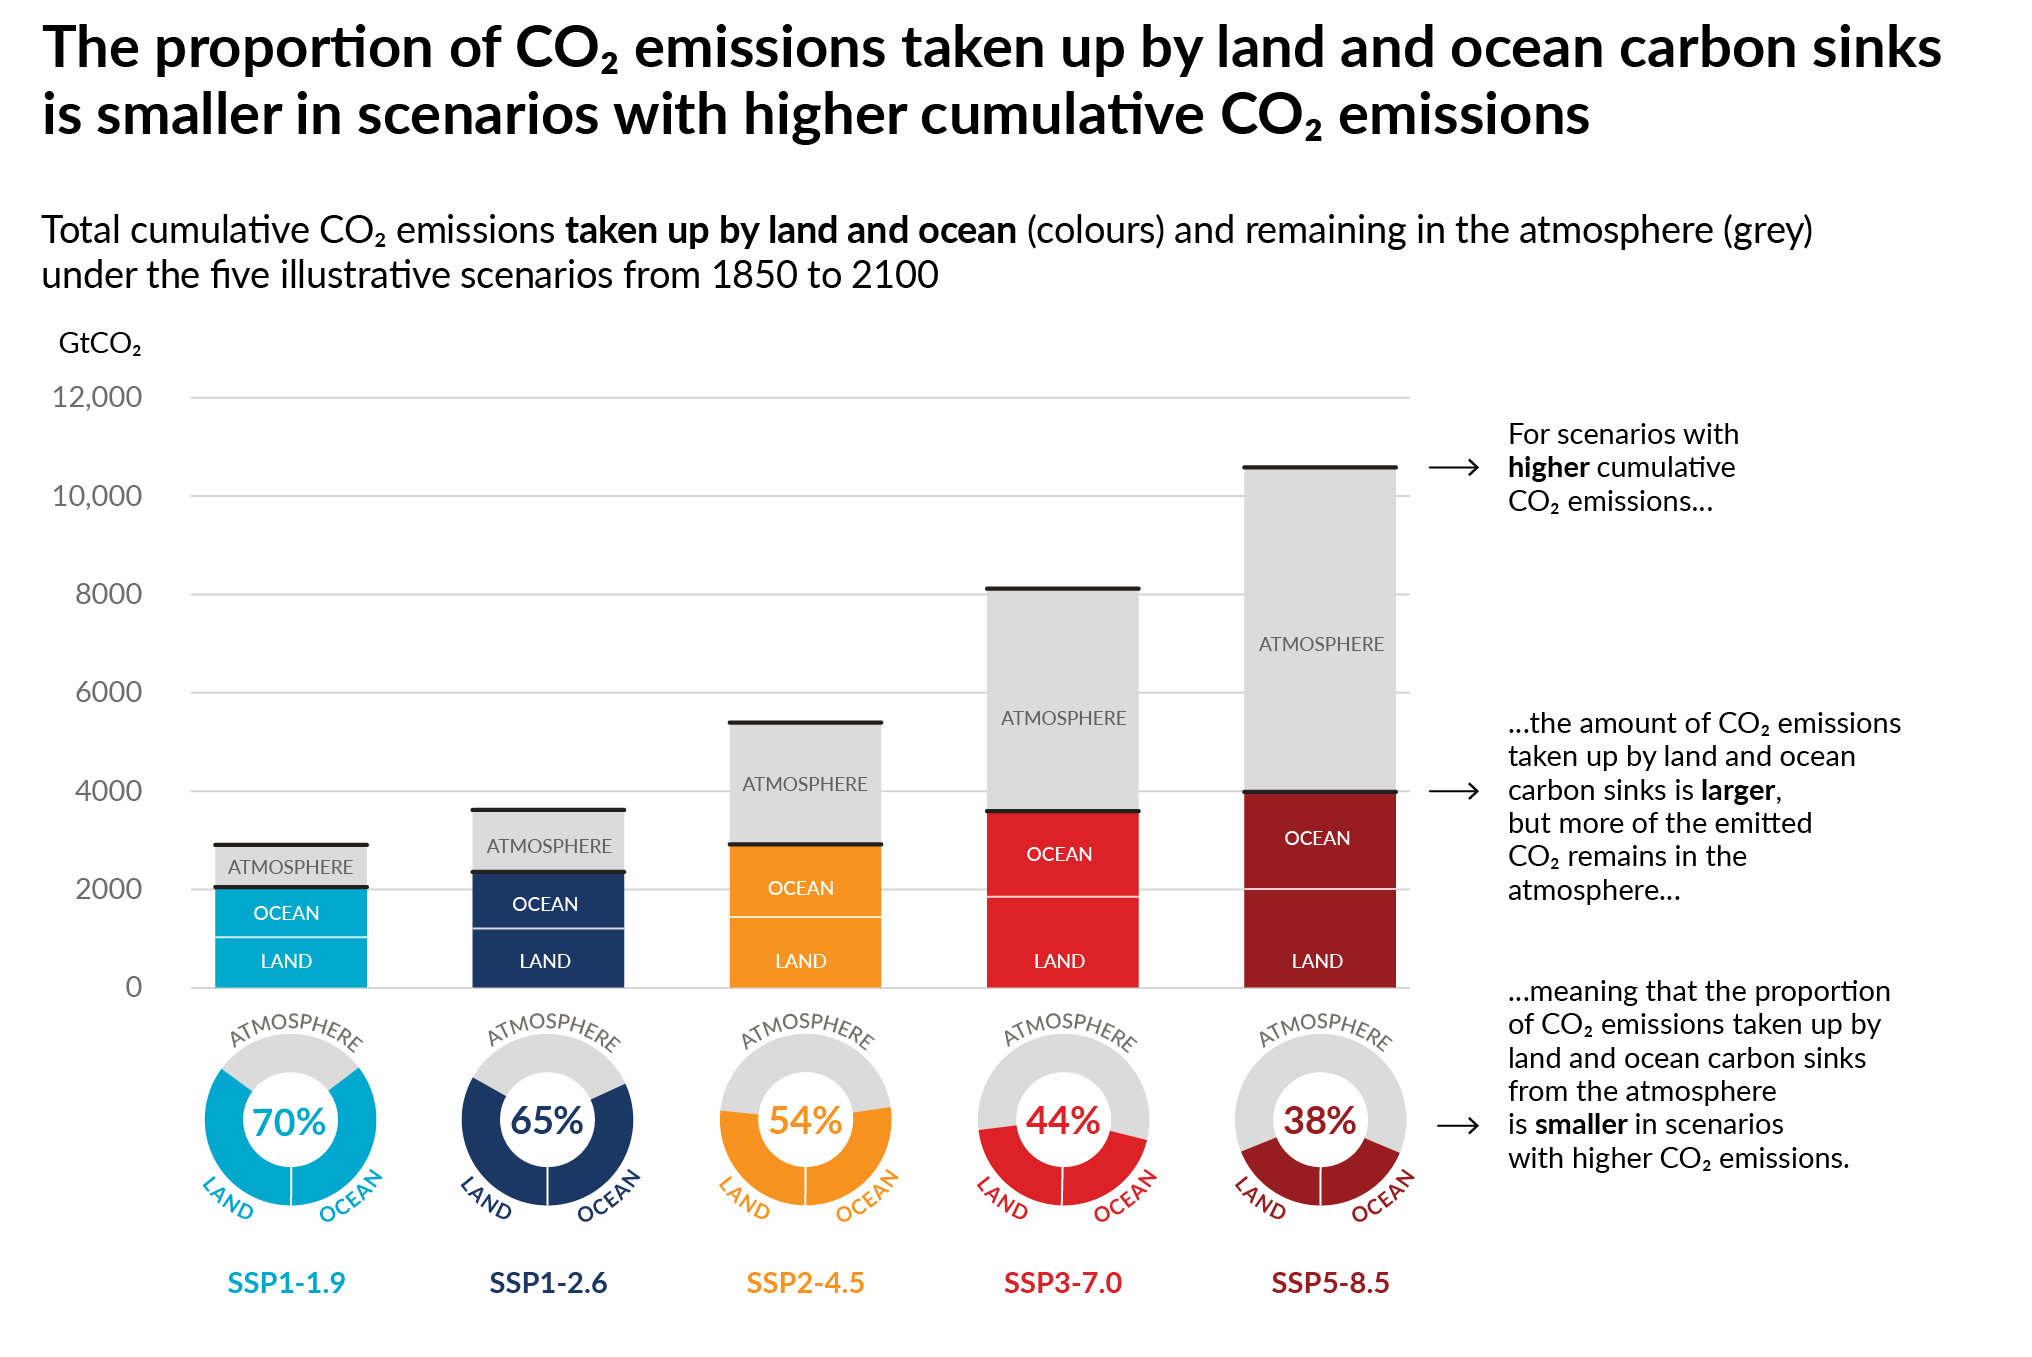
\includegraphics[width=\linewidth, totalheight=0.82\textheight, keepaspectratio]{future-SPM_Figure_7.png}
    \slidereference{IPCC AR6, SPM}
\end{frame}

\begin{frame}{Commitments}
    \centering
    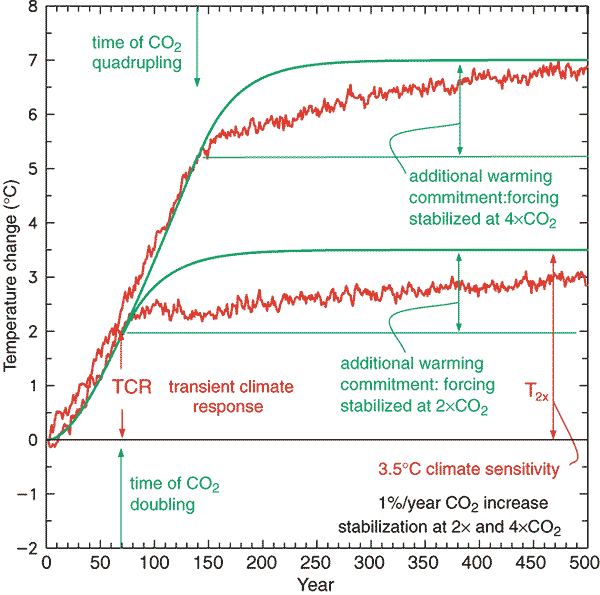
\includegraphics[width=\linewidth, totalheight=0.75\textheight, keepaspectratio]{future-TCR-ECS-AR3.png}
    \slidereference{IPCC AR3}
\end{frame}

\section{Climate Sensitivity}

\begin{frame}{Climate Sensitivity}
    \centering
    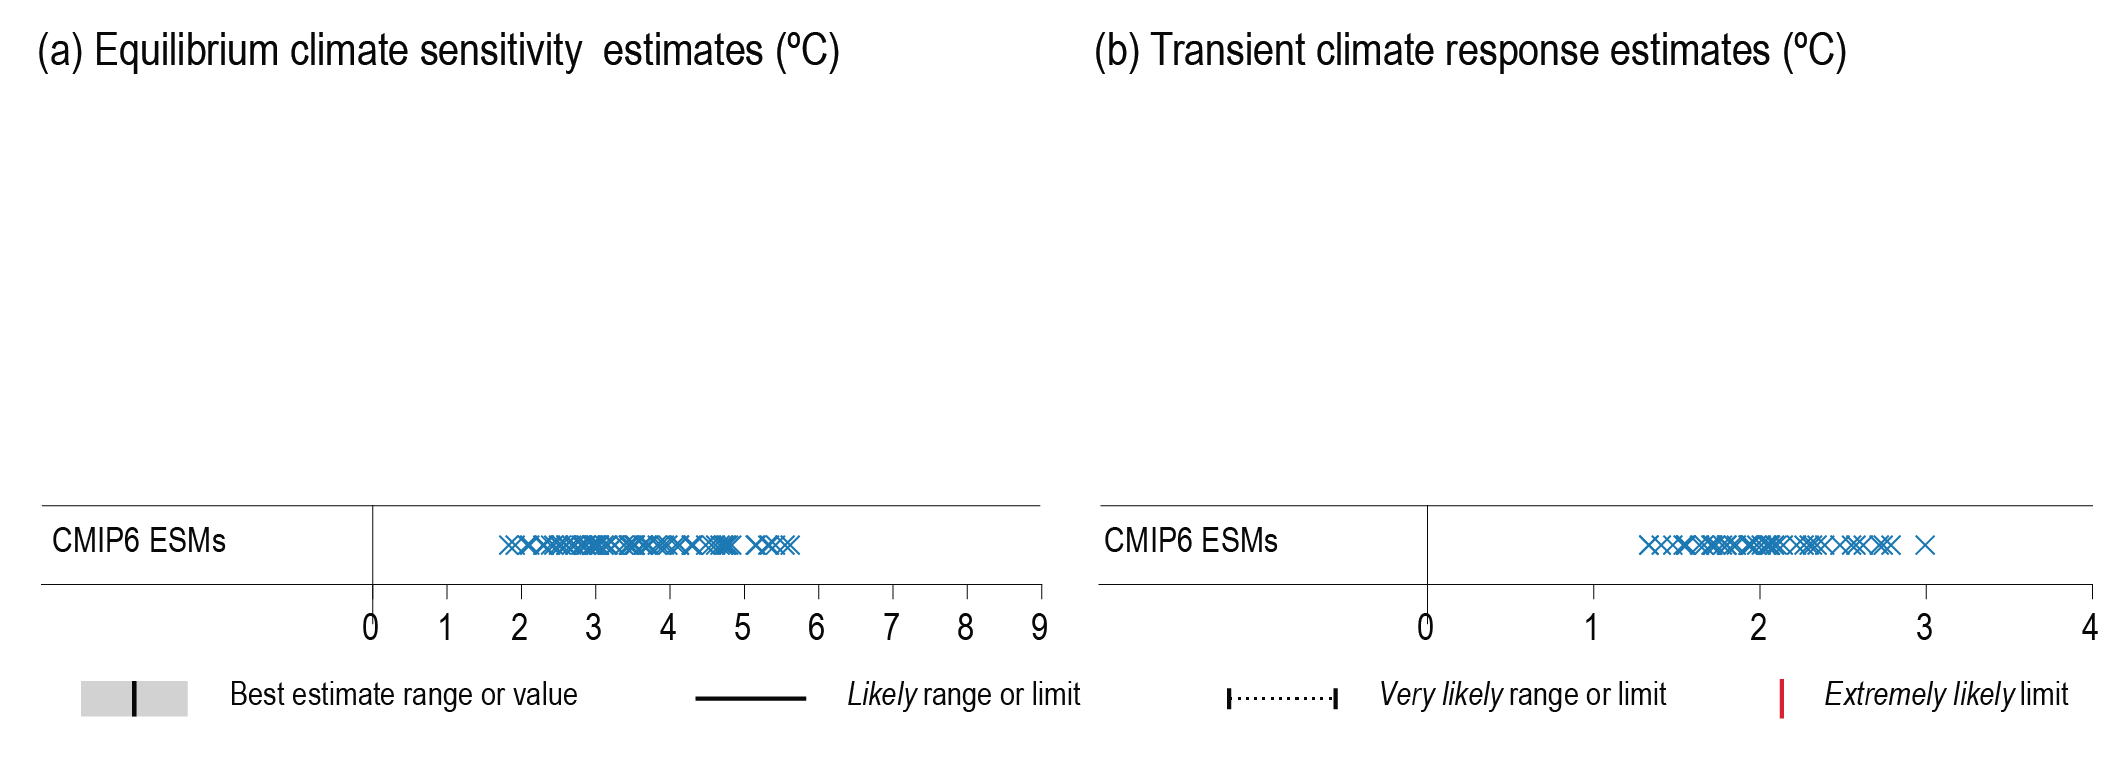
\includegraphics[width=\linewidth, totalheight=0.75\textheight, keepaspectratio]{future-AR6_WGI_Figure_7_18.0.png}
    \slidereference{IPCC AR6}
\end{frame}


% https://www.carbonbrief.org/explainer-how-scientists-estimate-climate-sensitivity/

% \begin{frame}{Climate Sensitivity}
%     \centering
%     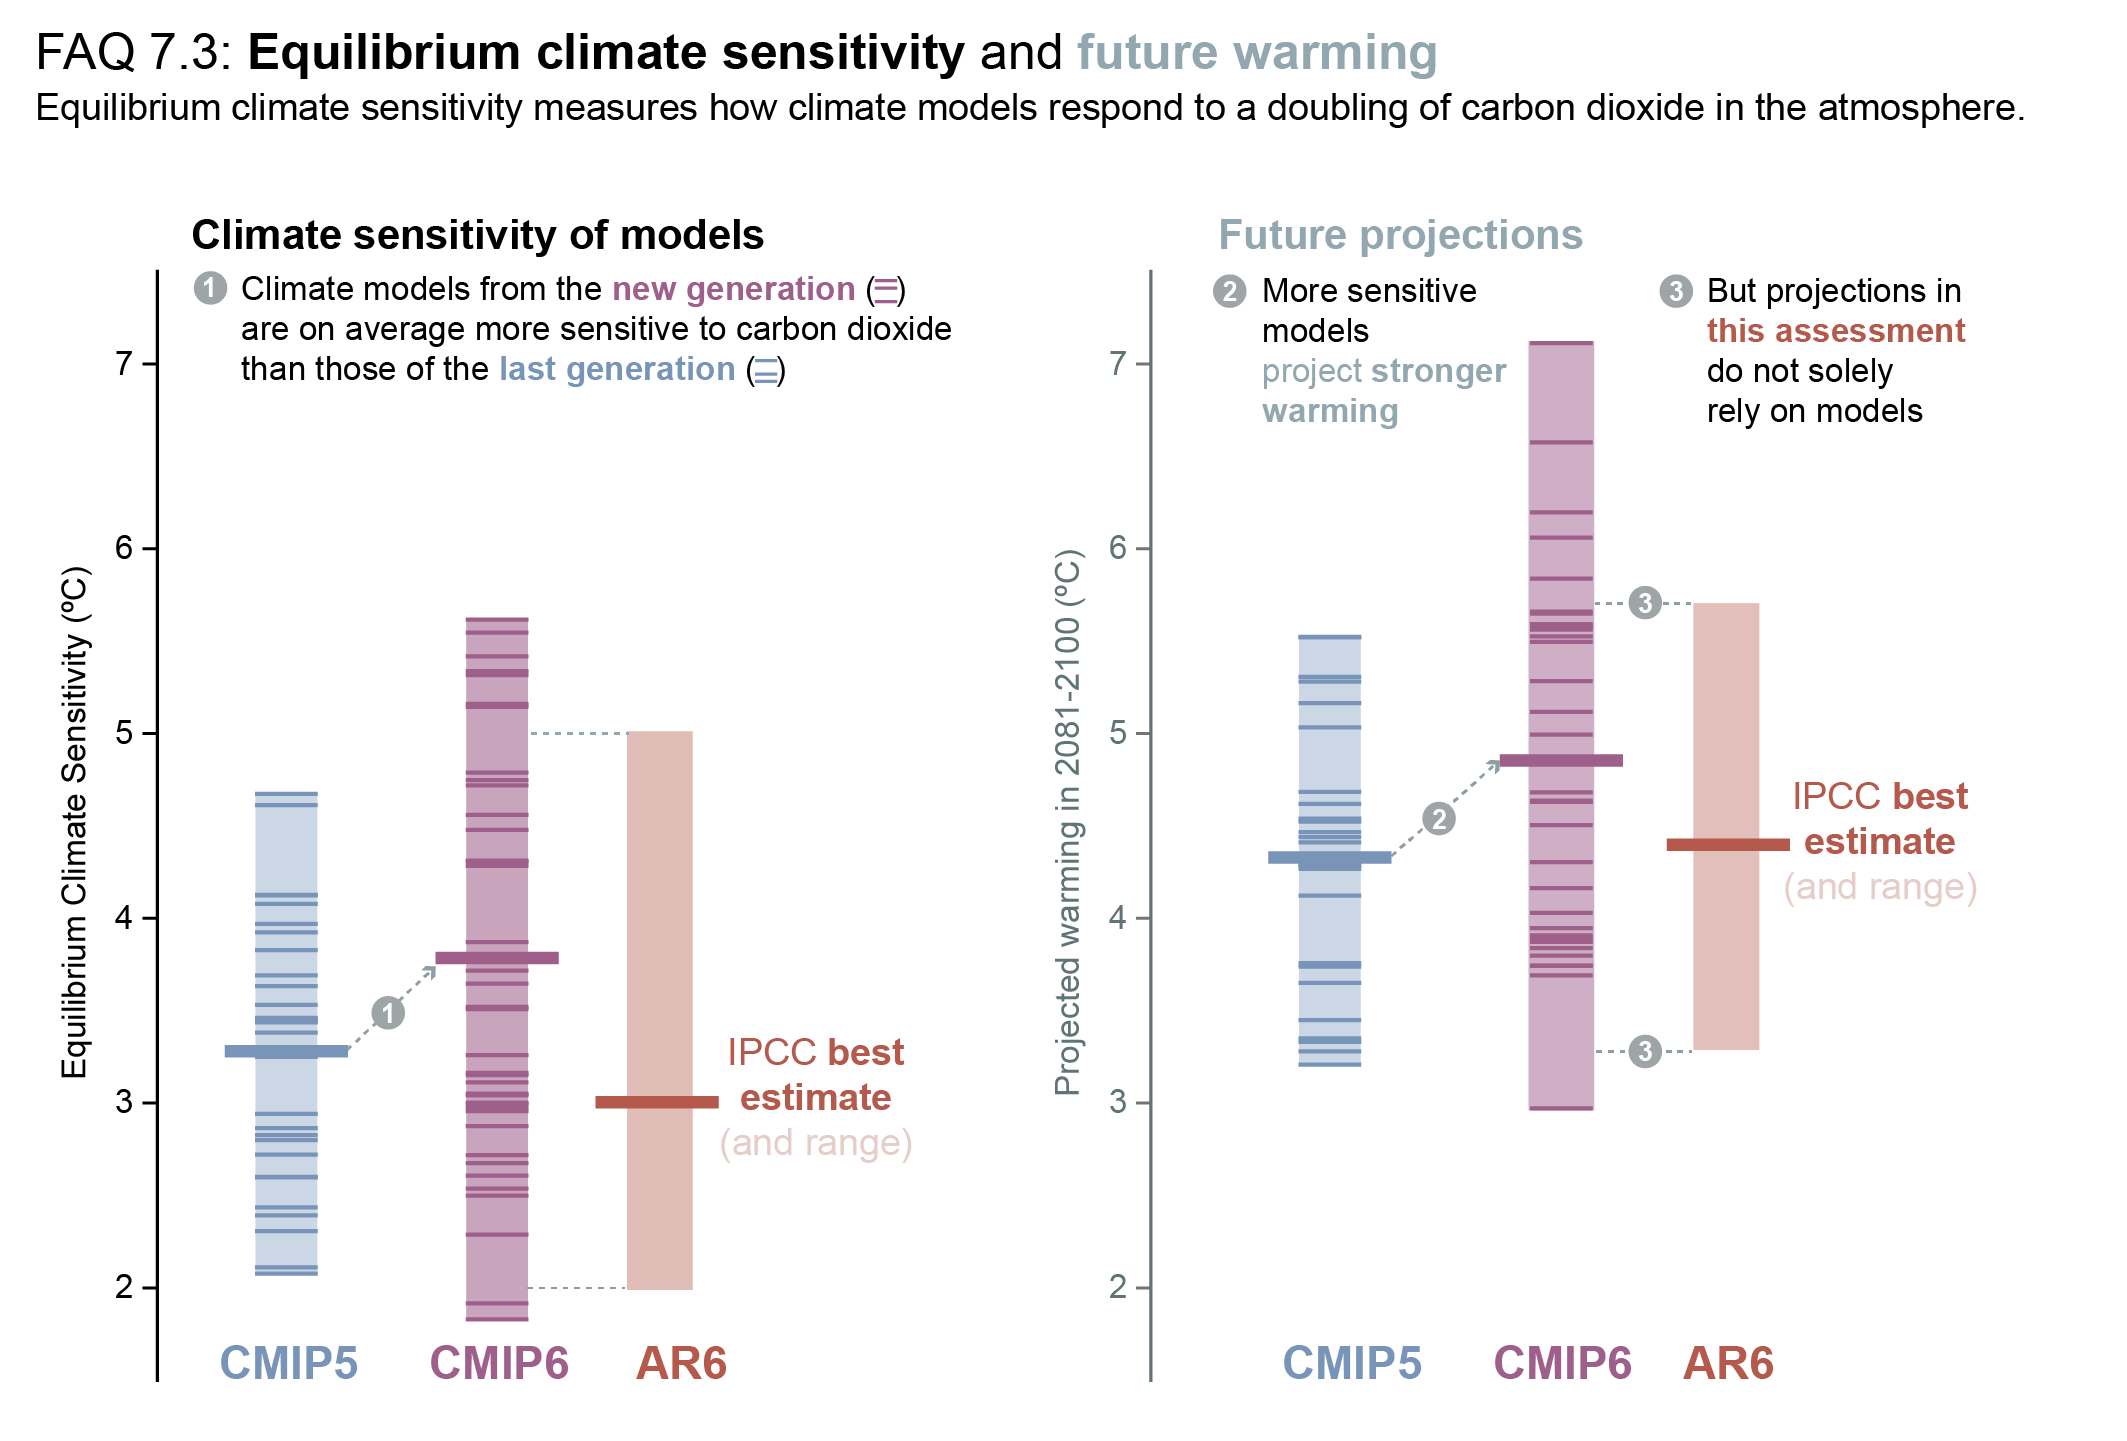
\includegraphics[width=\linewidth, totalheight=0.75\textheight, keepaspectratio]{future-model-sensitivity.png}
%     \slidereference{IPCC AR6}
% \end{frame}

\begin{frame}{Can we use models to estimate sensitivity?}
    \centering
    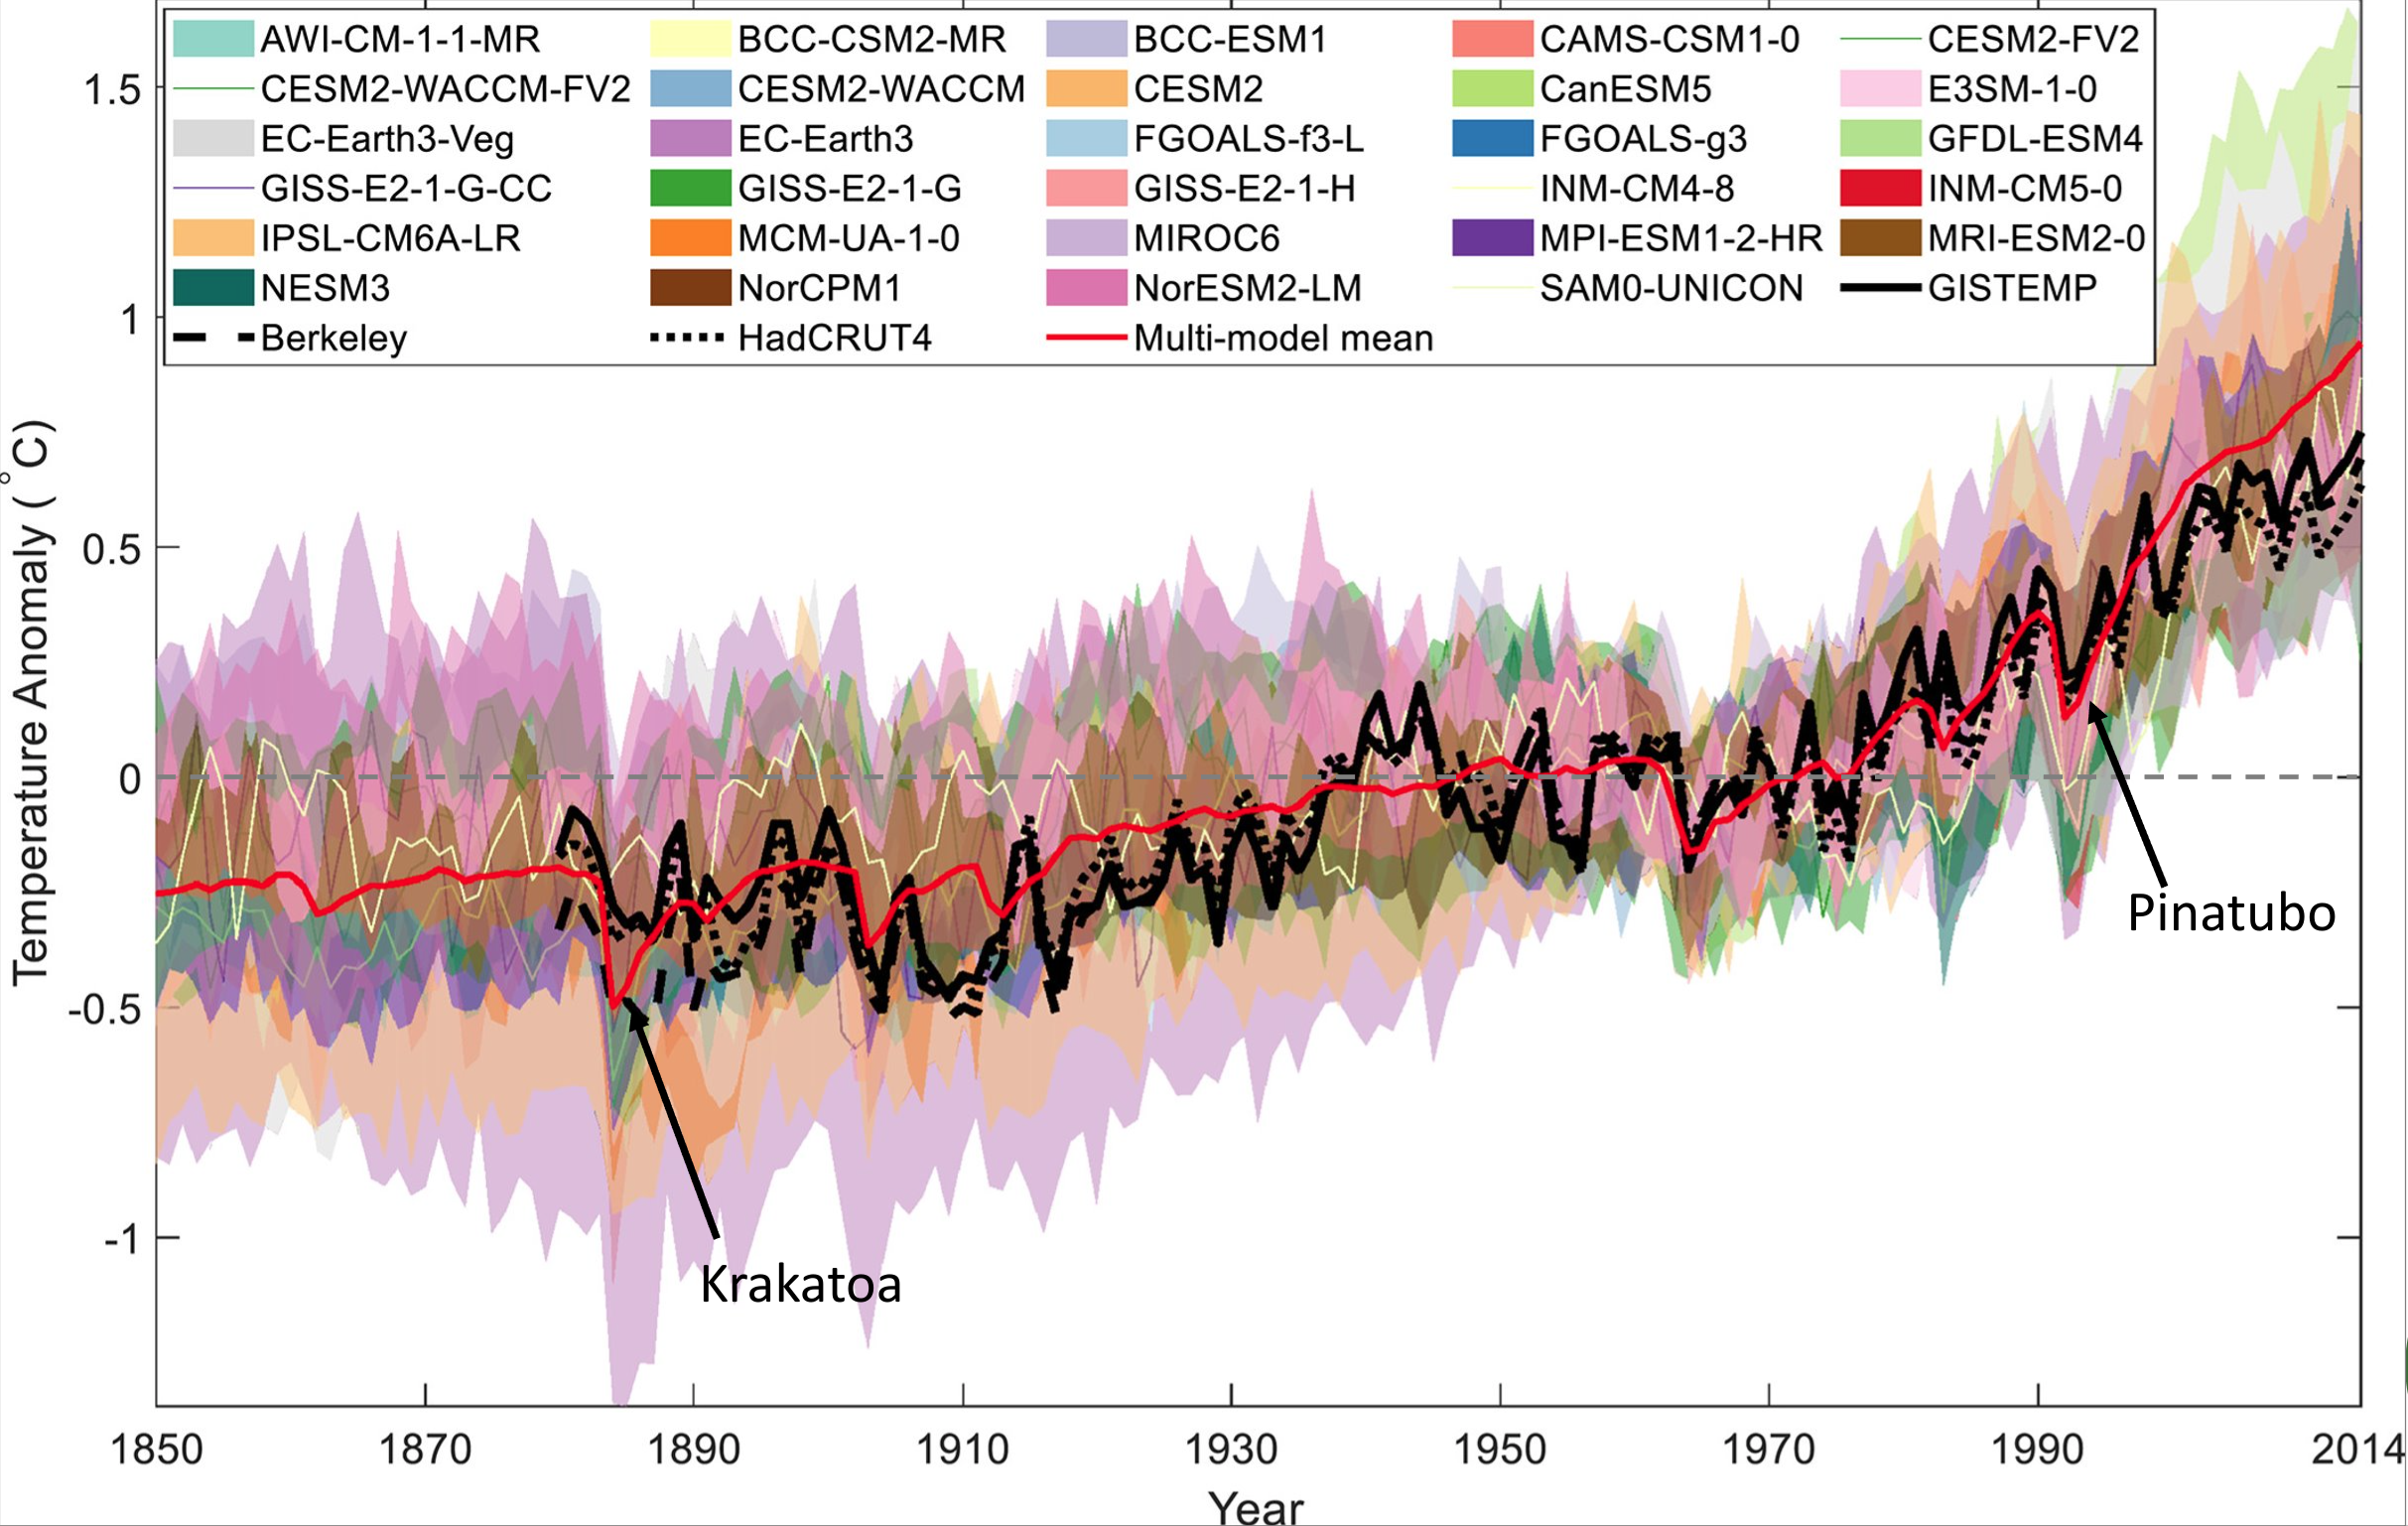
\includegraphics[width=\linewidth, totalheight=0.75\textheight, keepaspectratio]{future-model-hindcast.png}

    % But IPCC models are 'ground truthed' against the modern world... (narrow range of conditions, hindcast figure)    
    % Complex feedbacks (Alex's Fig)

\end{frame}

\begin{frame}{Transient Climate Response}
    \centering
    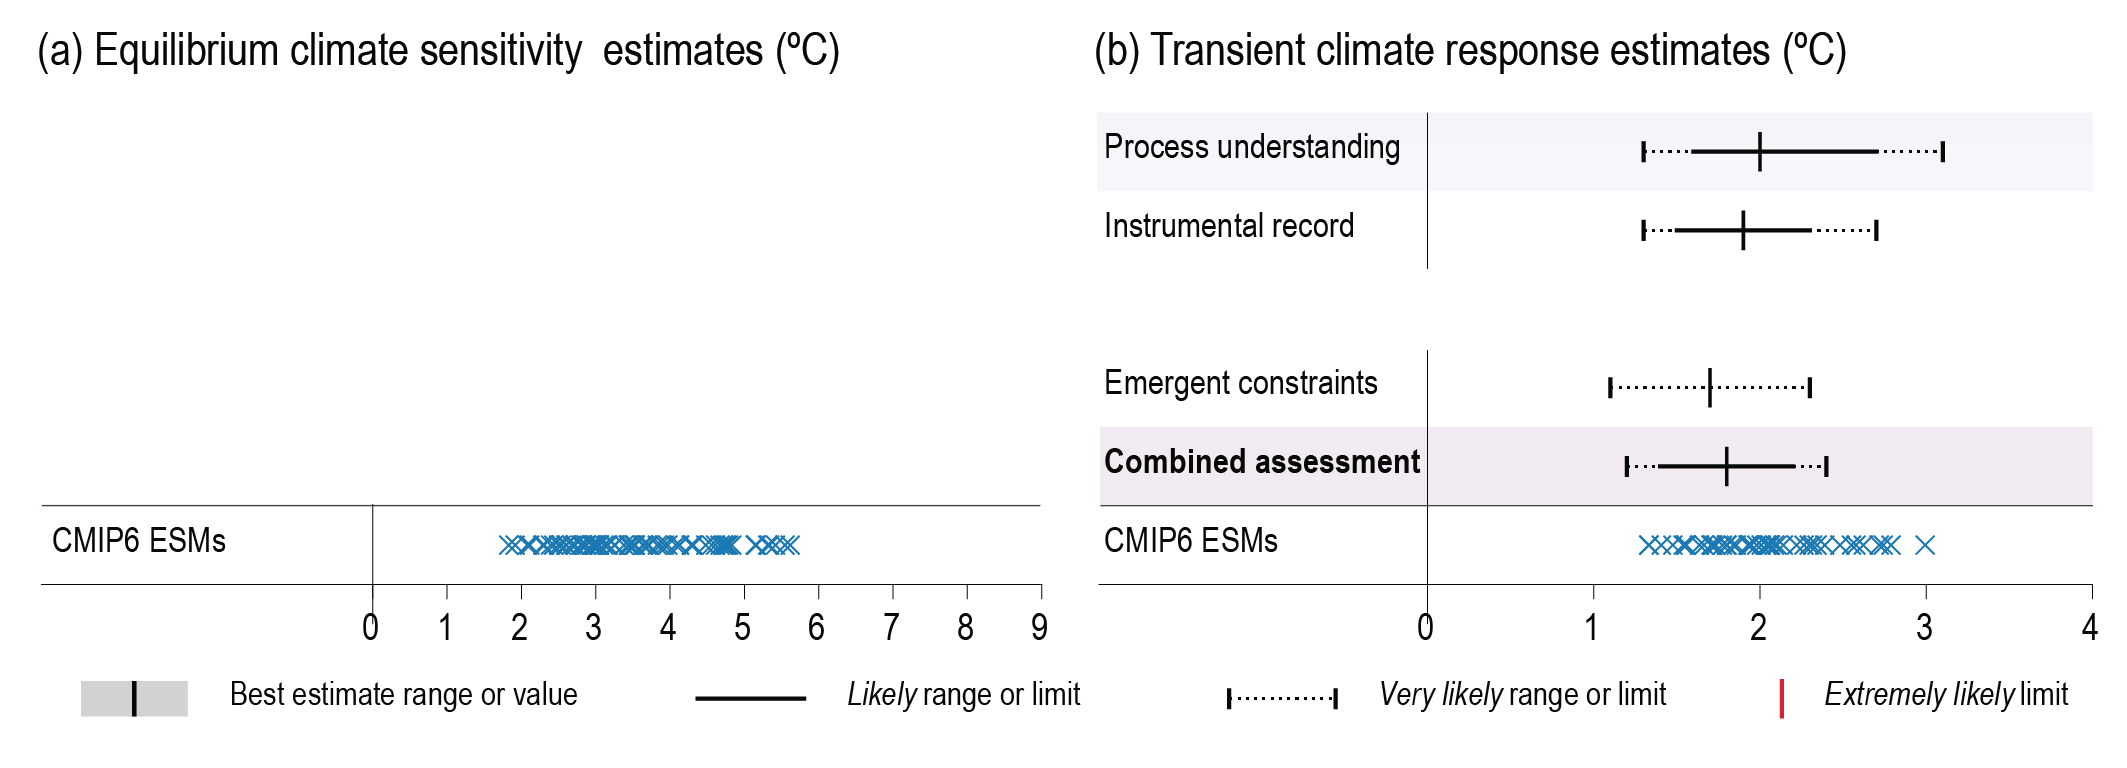
\includegraphics[width=\linewidth, totalheight=0.75\textheight, keepaspectratio]{future-AR6_WGI_Figure_7_18.1.png}
    \slidereference{IPCC AR6}
\end{frame}

\begin{frame}{Transient Climate Response}
    \centering
    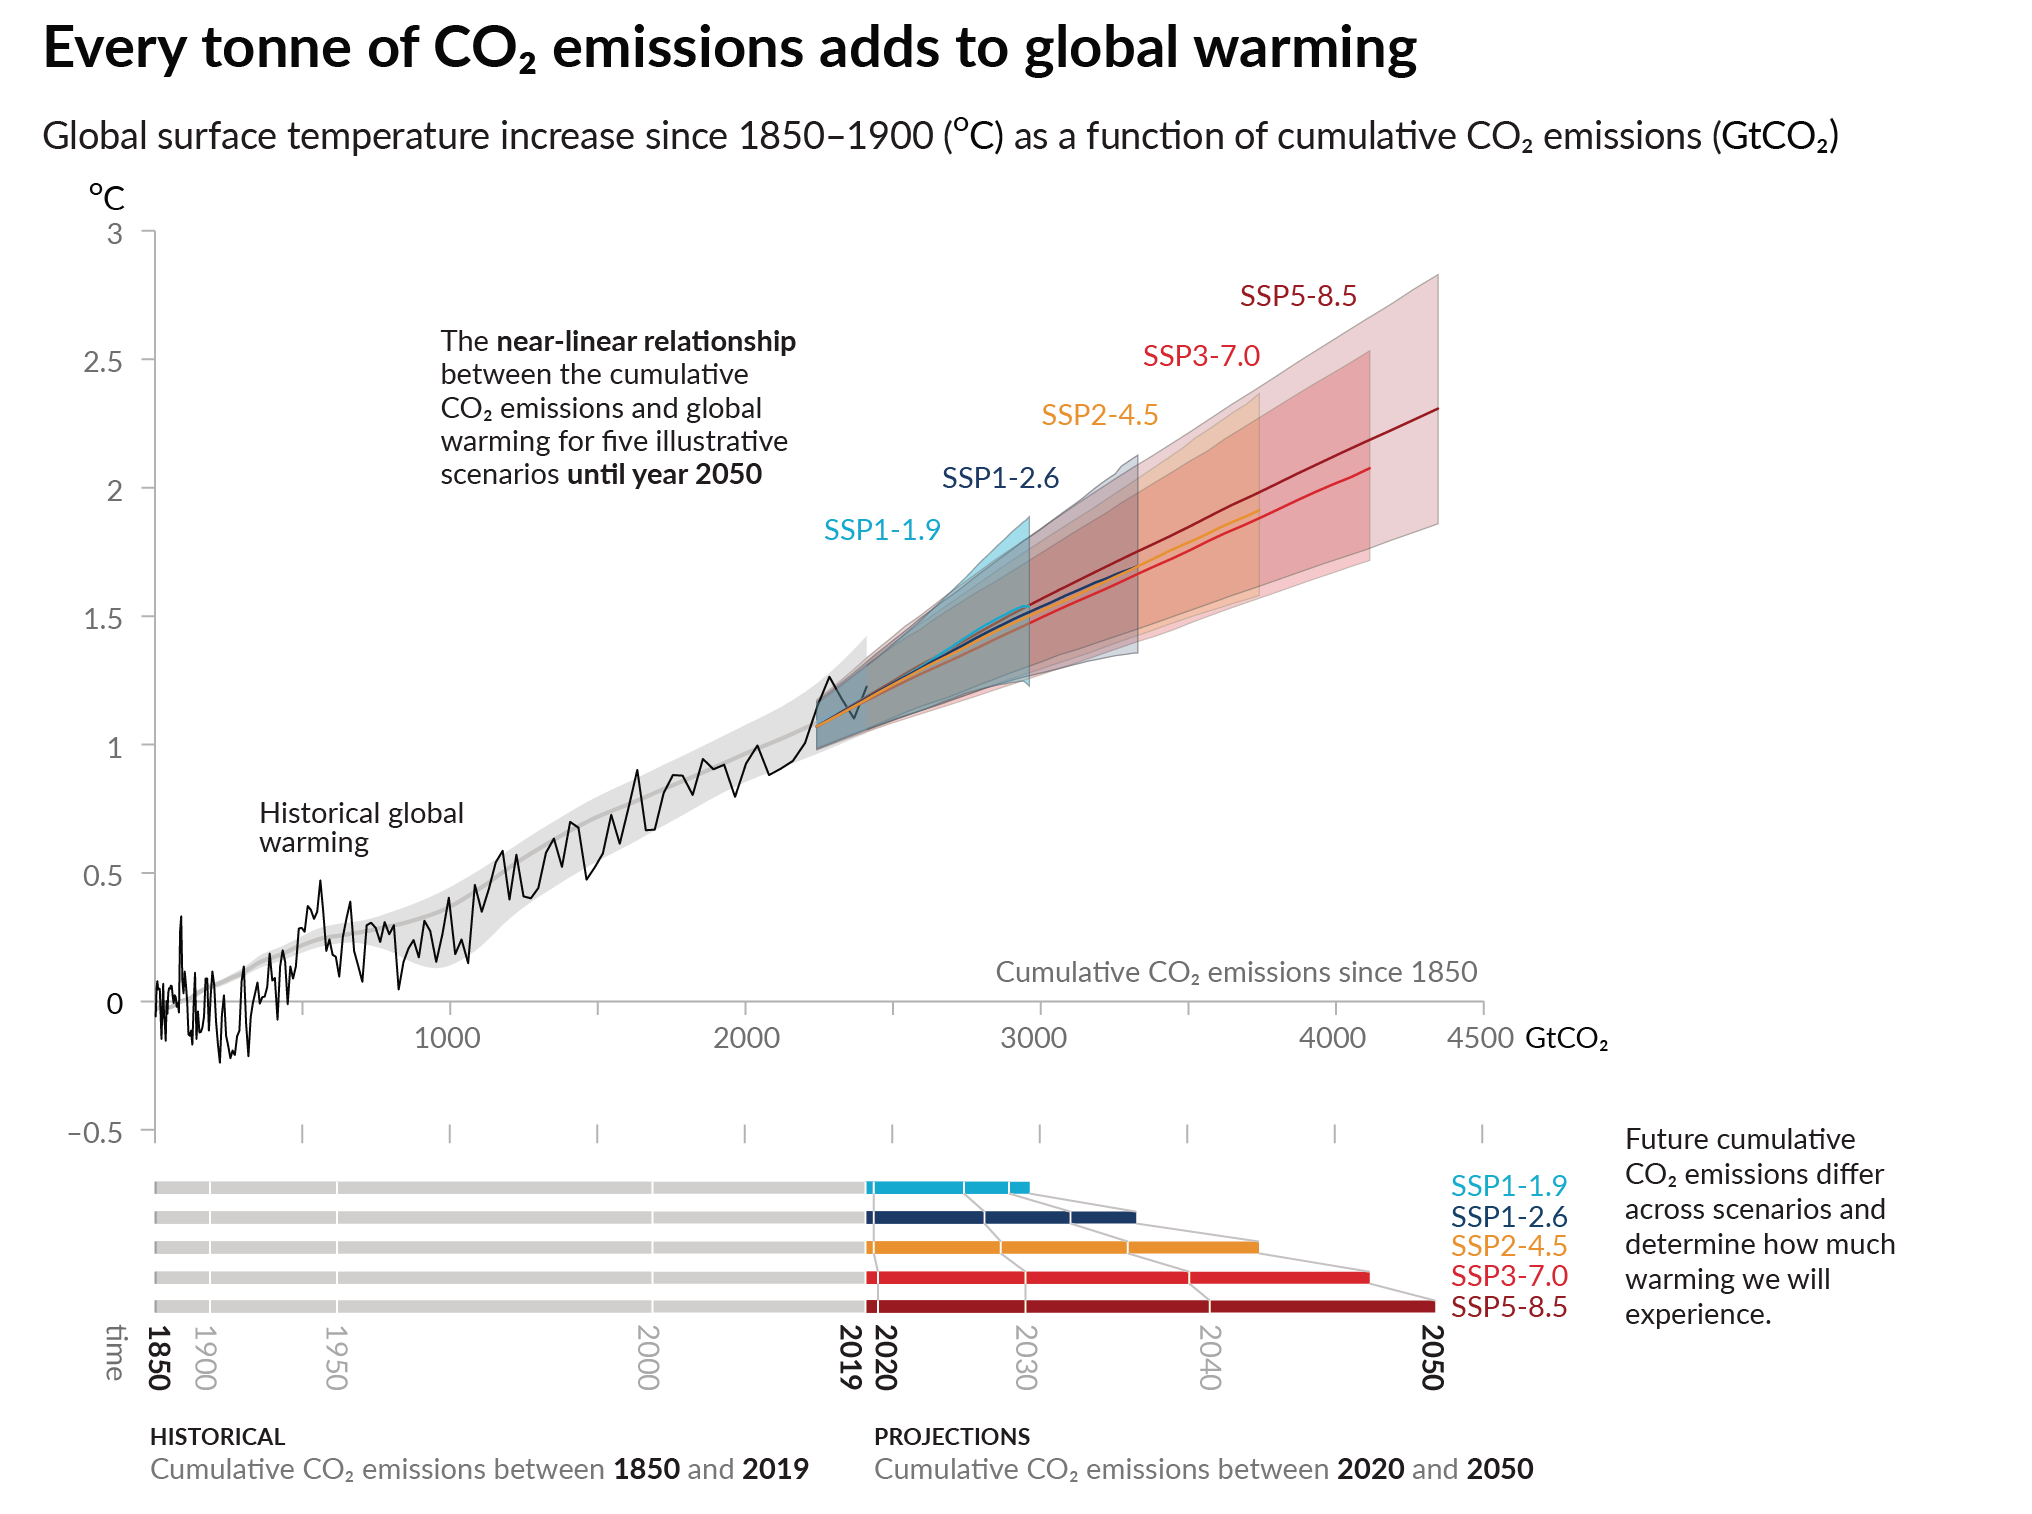
\includegraphics[width=\linewidth, totalheight=0.82\textheight, keepaspectratio]{future-SPM_Figure_10.png}
    \slidereference{IPCC AR6, SPM}
\end{frame}

\begin{frame}{Equilibrium Climate Sensitivity?}
    \centering
    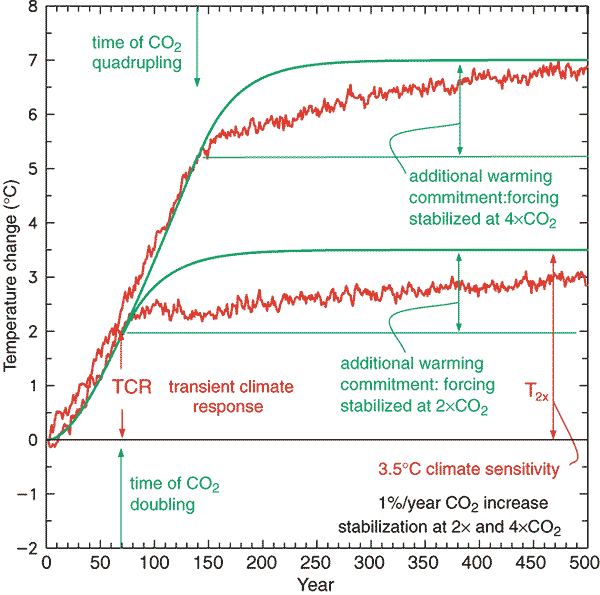
\includegraphics[width=\linewidth, totalheight=0.75\textheight, keepaspectratio]{future-TCR-ECS-AR3.png}
    \slidereference{IPCC AR3}
\end{frame}

\begin{frame}{Feedback Timescales}
    \centering
    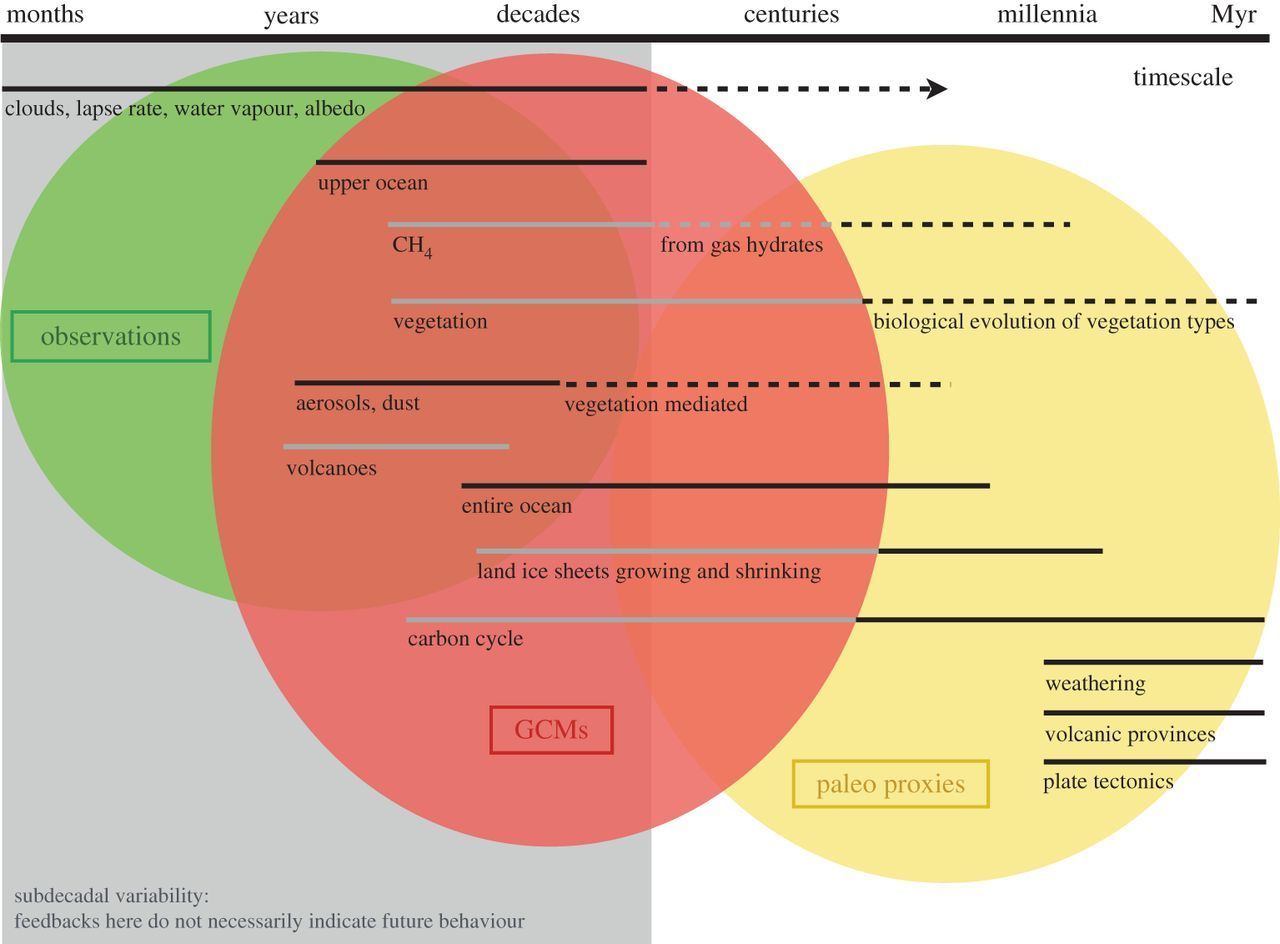
\includegraphics[width=\linewidth, totalheight=0.75\textheight, keepaspectratio]{future-feedback-timescales.jpg}
    \slidereference{Knutti \& Rugenstein, 2015}
\end{frame}

\begin{frame}{Equilibrium Climate Sensitivity}
    \centering
    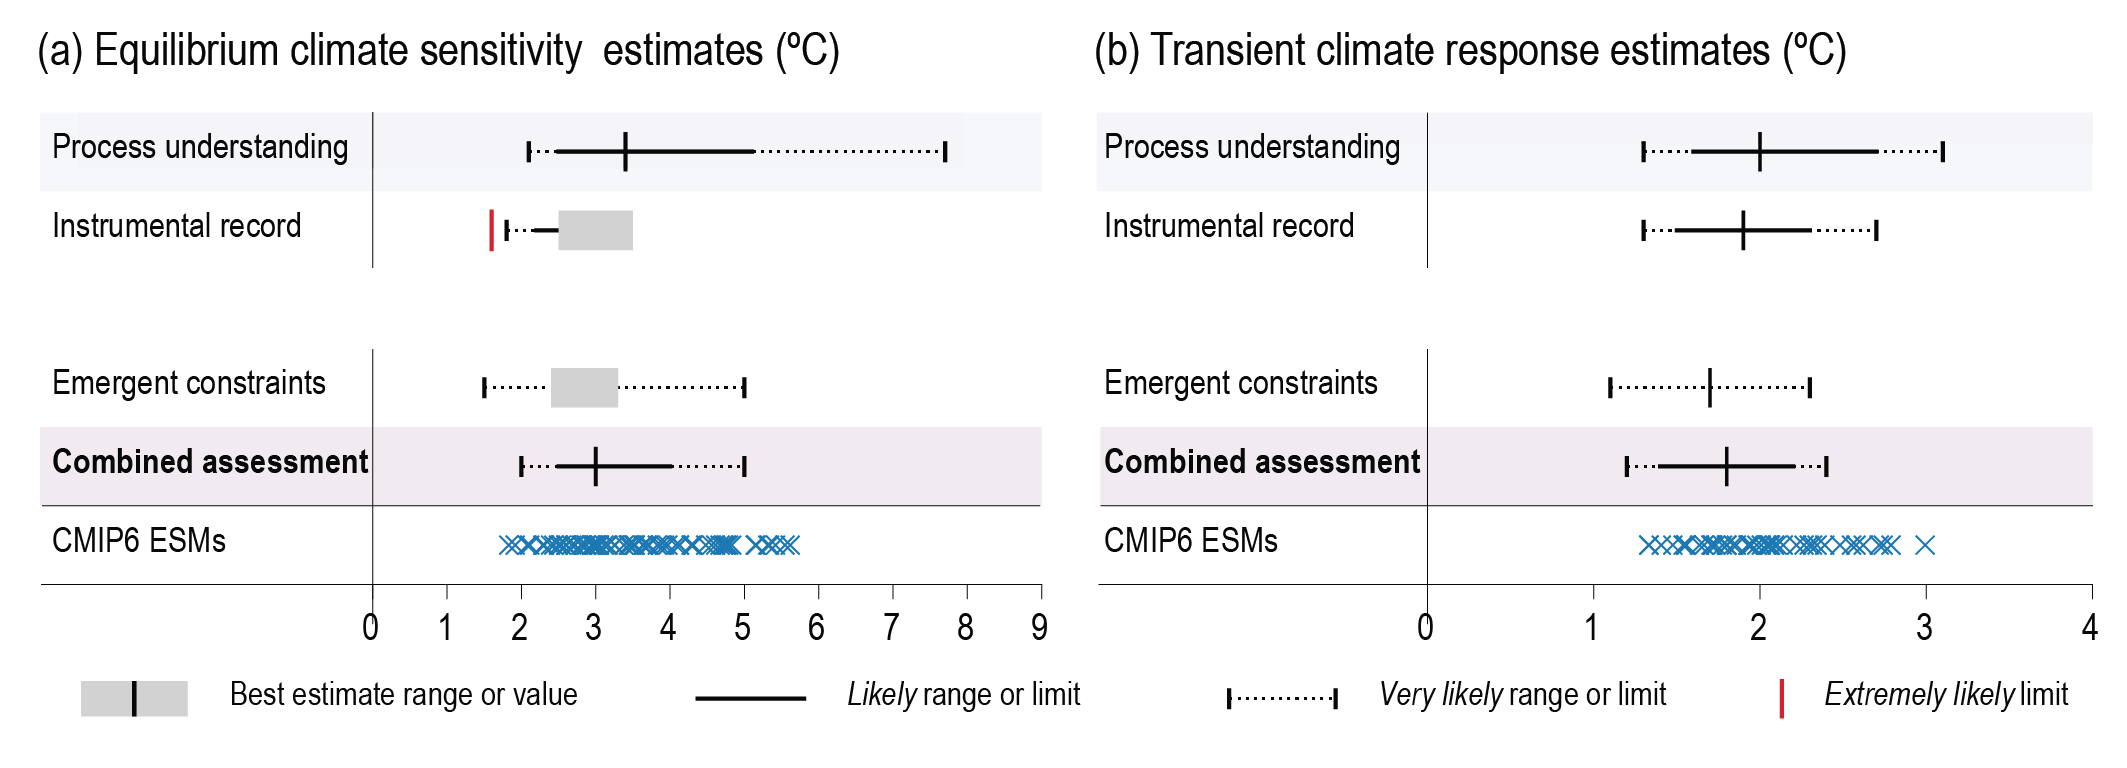
\includegraphics[width=\linewidth, totalheight=0.75\textheight, keepaspectratio]{future-AR6_WGI_Figure_7_18.2.png}
    \slidereference{IPCC AR6}
\end{frame}

\begin{frame}{Precedent?}
    % we are pushing the climate into an unknown regime.
    \centering
    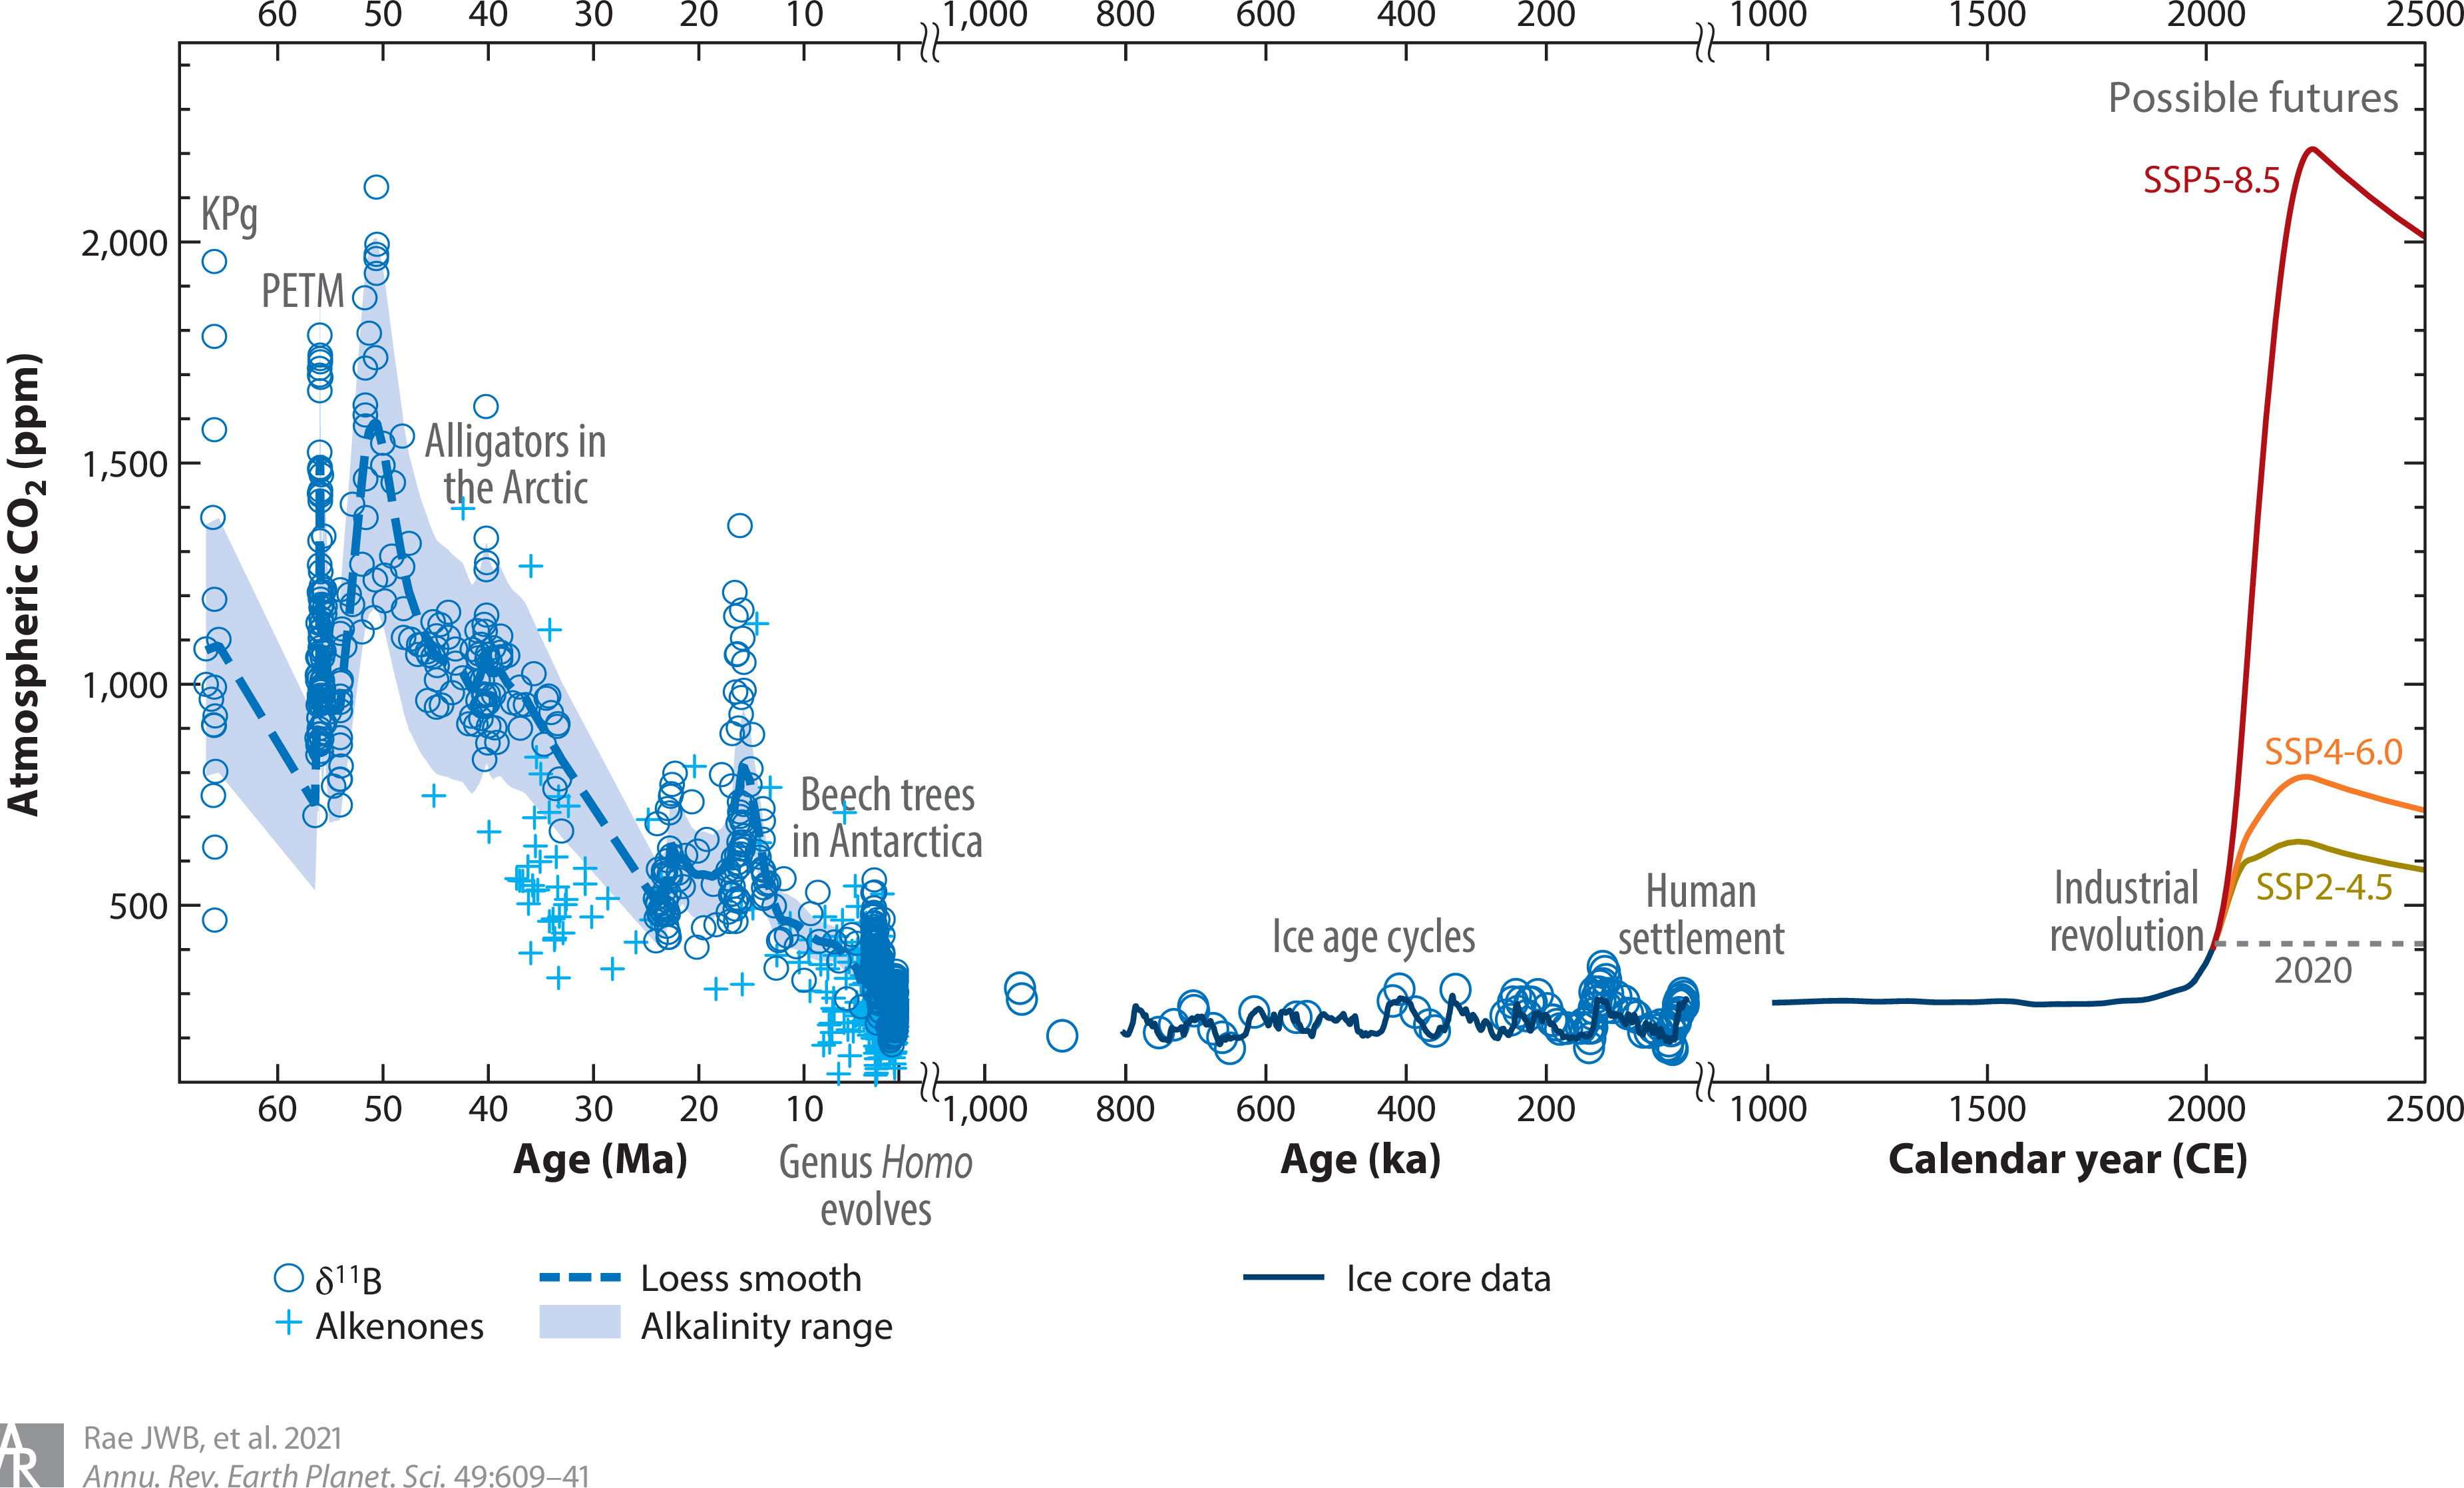
\includegraphics[width=\linewidth, totalheight=0.8\textheight, keepaspectratio]{future-palaeo-co2.jpeg}
\end{frame}            

\section{Past Climate}

\begin{frame}{Climate Records}
    % how do we know what happened in past climates?
    % palaeo-CO2
    % palaeo-temperature
\end{frame}

\begin{frame}{Palaeo-\ce{pCO2}}
    % how do we know what happened in past climates?
    % palaeo-CO2
    % palaeo-temperature
\end{frame}

\begin{frame}{Palaeo-Temperature}
    % how do we know what happened in past climates?
    % palaeo-CO2
    % palaeo-temperature
\end{frame}

\begin{frame}{Palaeo-Sensitivity}
    % palaeoclimate was more sensitive?
    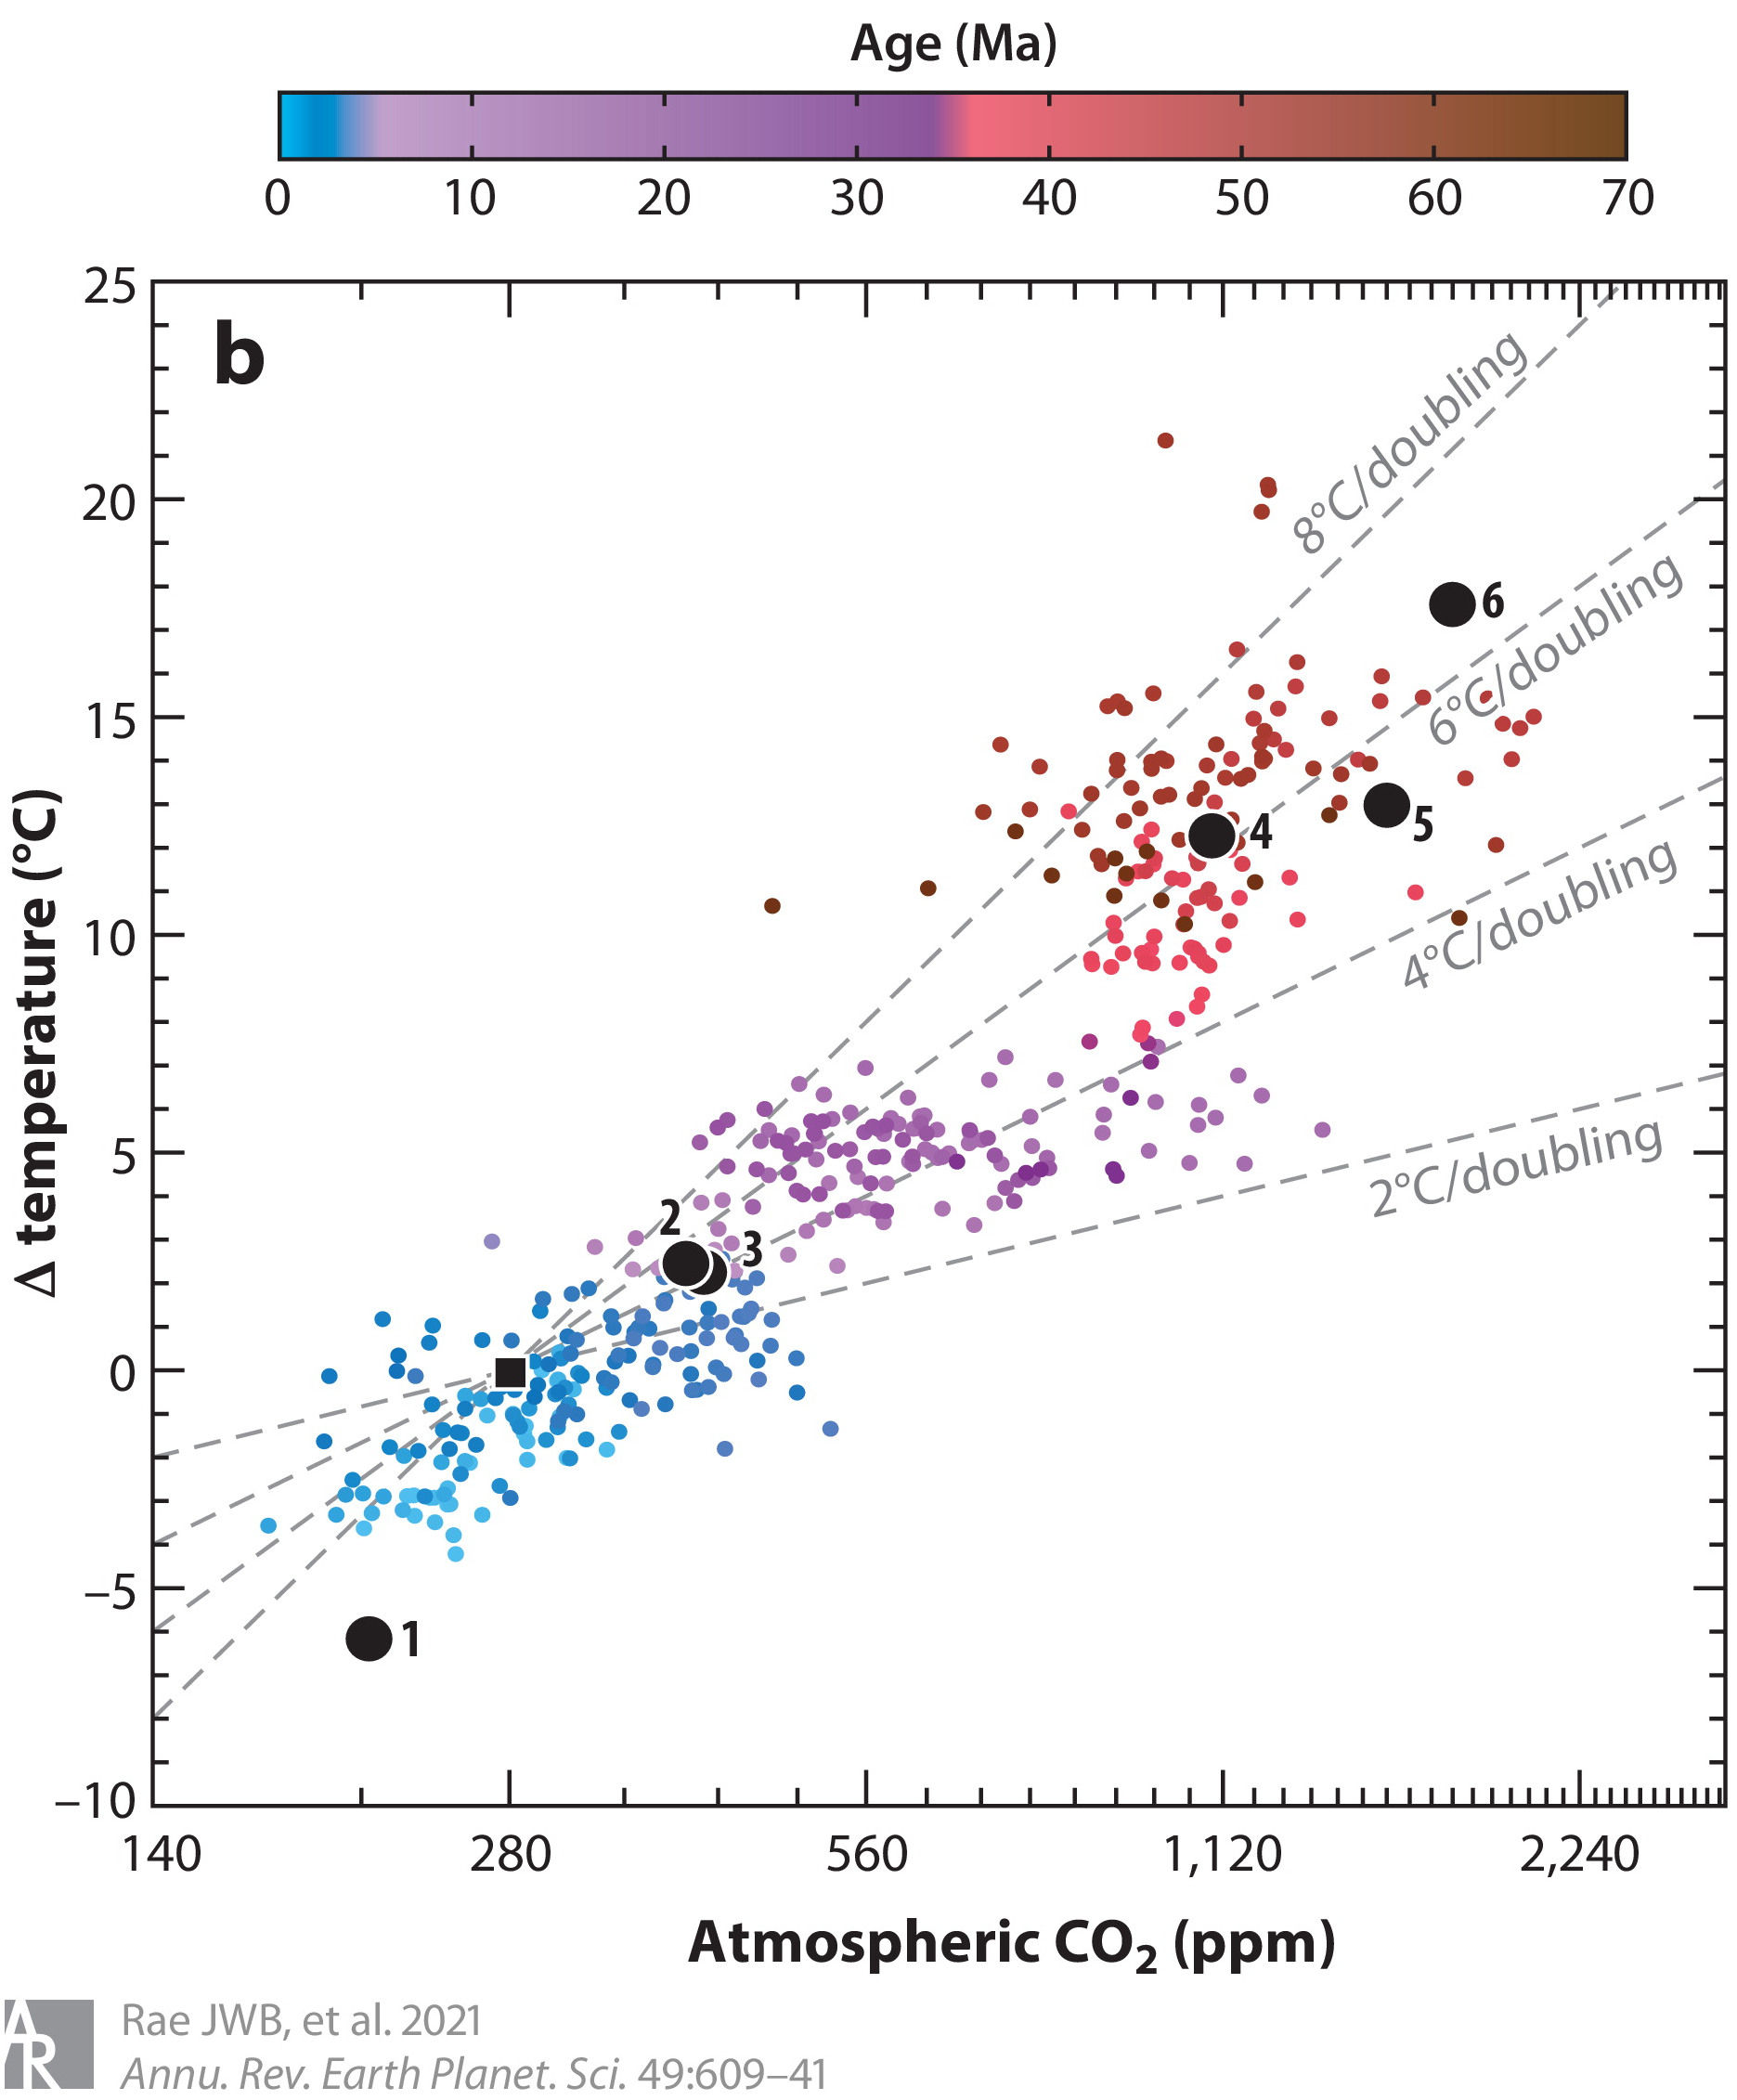
\includegraphics[width=\linewidth, totalheight=0.8\textheight, keepaspectratio]{future-palaeo-sensitivity.jpeg}
\end{frame}

\begin{frame}{Equilibrium Climate Sensitivity}
    \centering
    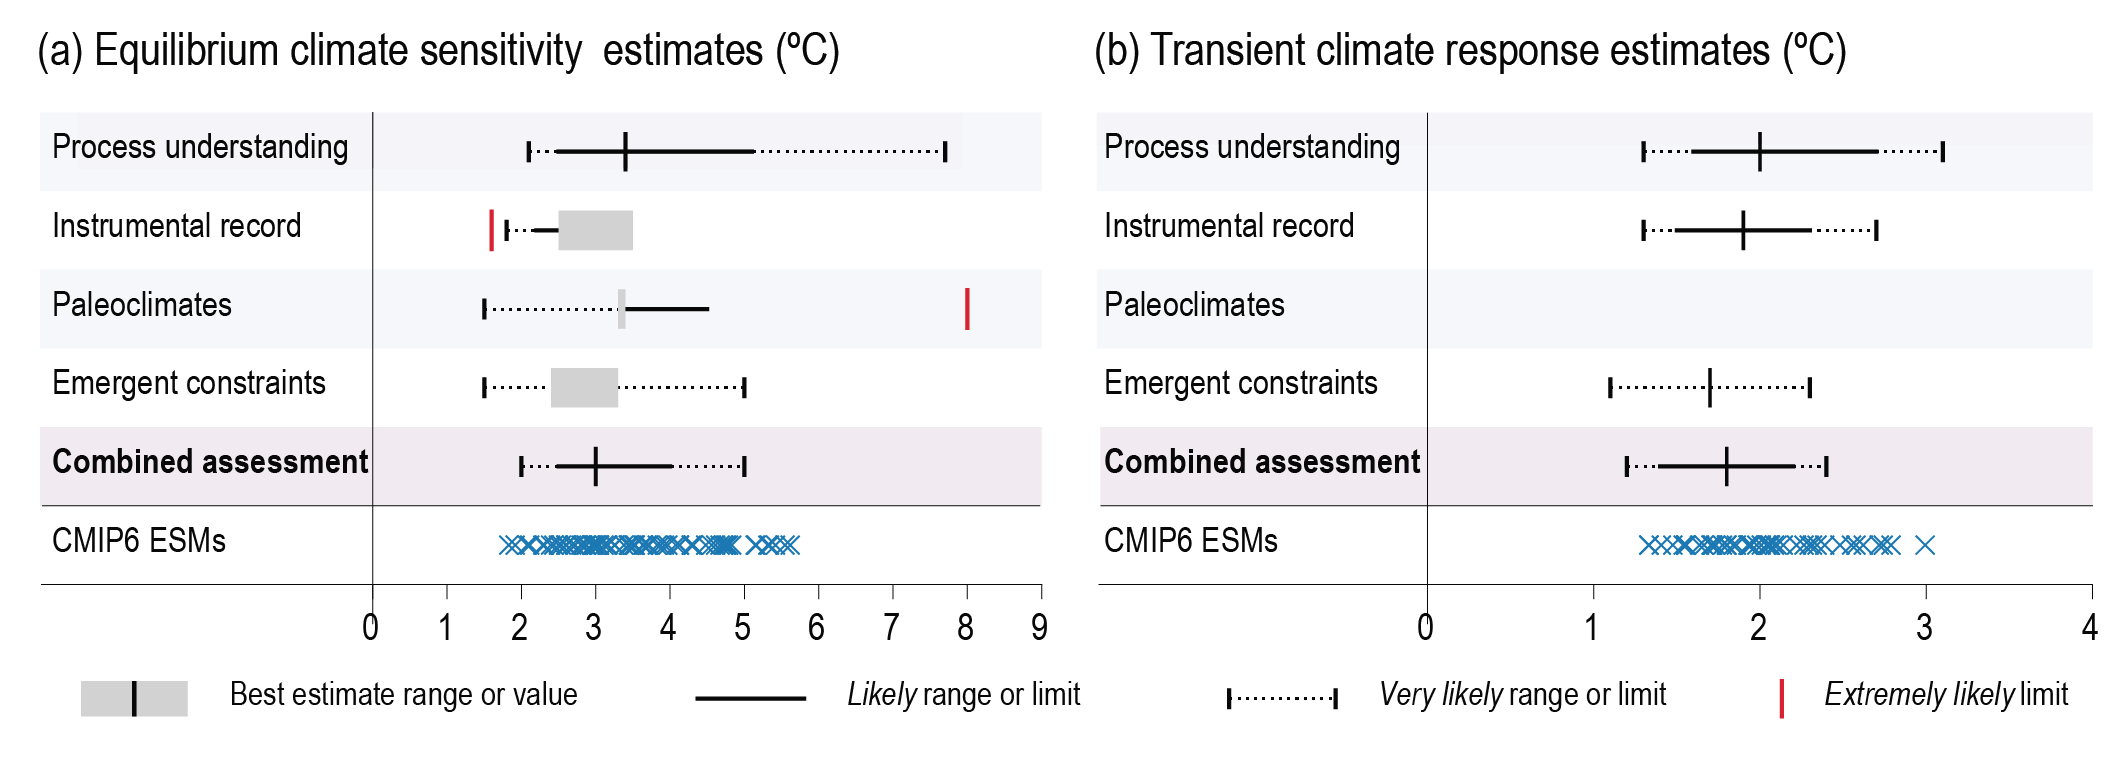
\includegraphics[width=\linewidth, totalheight=0.75\textheight, keepaspectratio]{future-AR6_WGI_Figure_7_18.png}
    \slidereference{IPCC AR6}

    \onslide<2|handout:1>{If we stop emitting now, temperatures will continue to rise by an uncertain amount (1.5-4x current warming).}
    % even if we stop emitting now, temperatures will rise for centuries, between 1.5-4x current warming.
\end{frame}

\section{Recovery}

\begin{frame}{Timescales of Recovery: PETM}
    \centering
    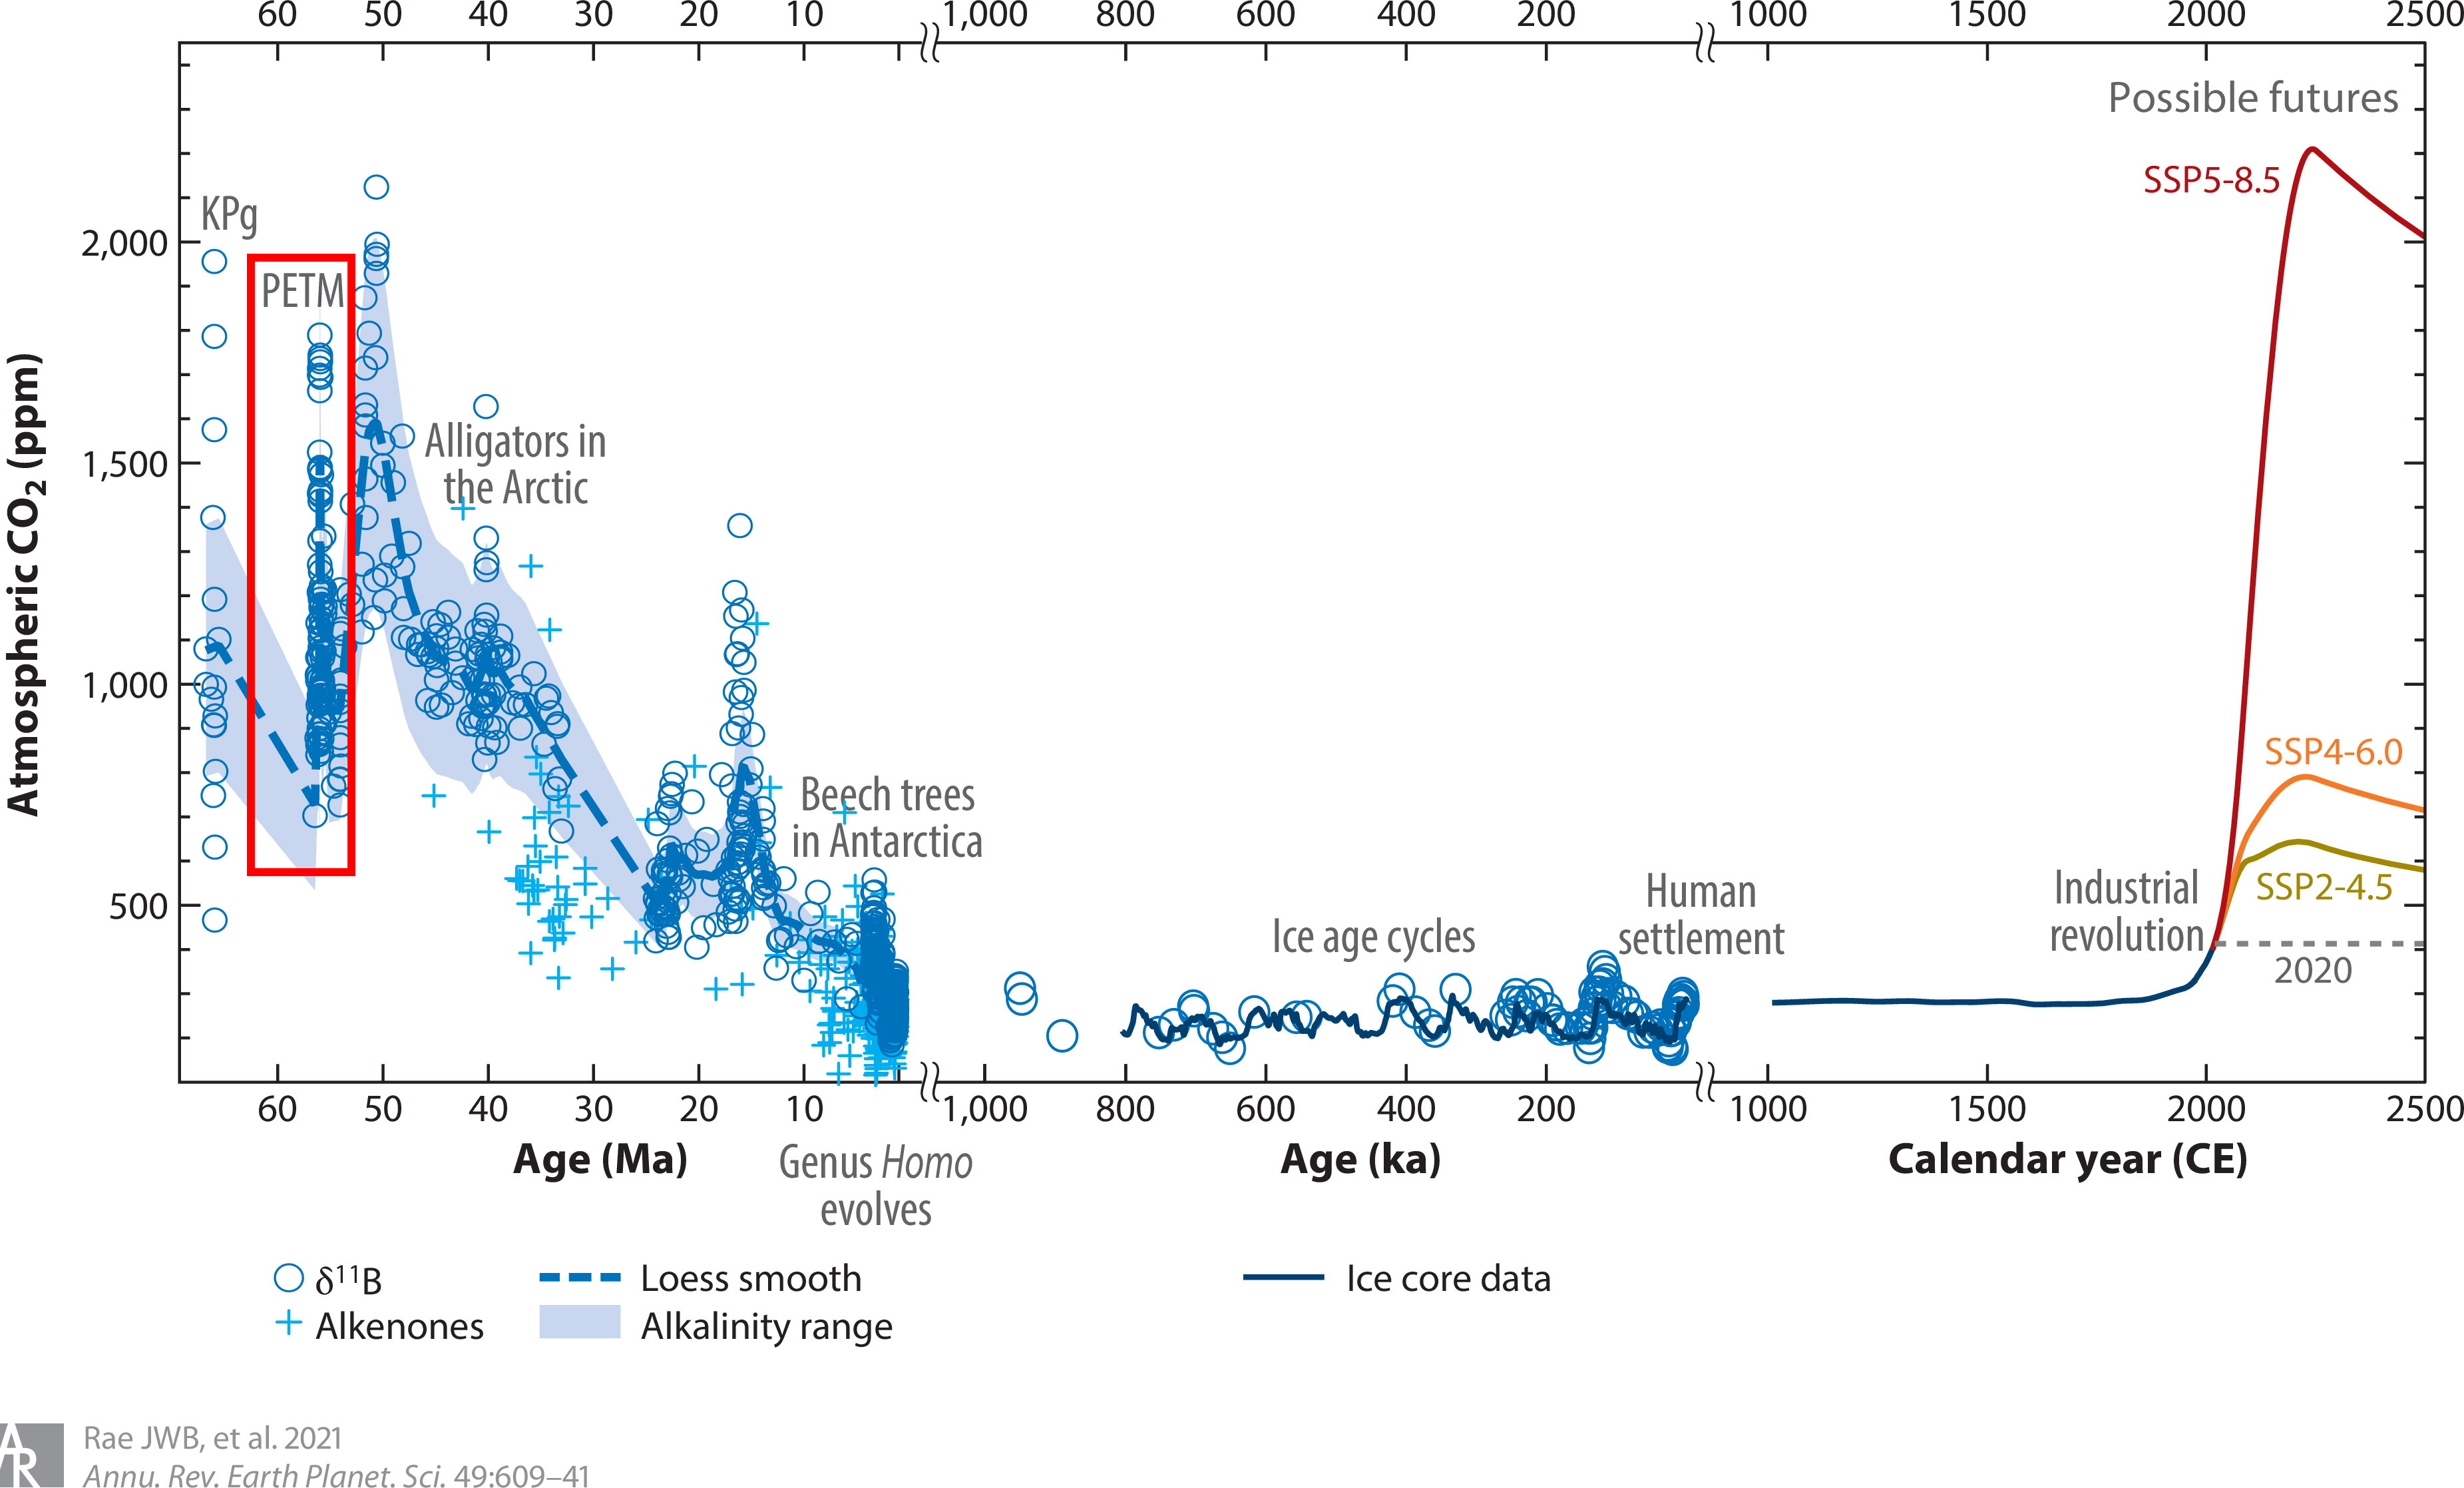
\includegraphics[width=\linewidth, totalheight=0.8\textheight, keepaspectratio]{future-palaeo-co2.1.jpeg}
\end{frame}

\begin{frame}{PETM: Mechanism?}

\end{frame}

\begin{frame}{PETM: Consequences}

\end{frame}

\begin{frame}{PETM: Recovery}

\end{frame}

\section{Urgency}

\begin{frame}{Urgent Action!}
    \centering
    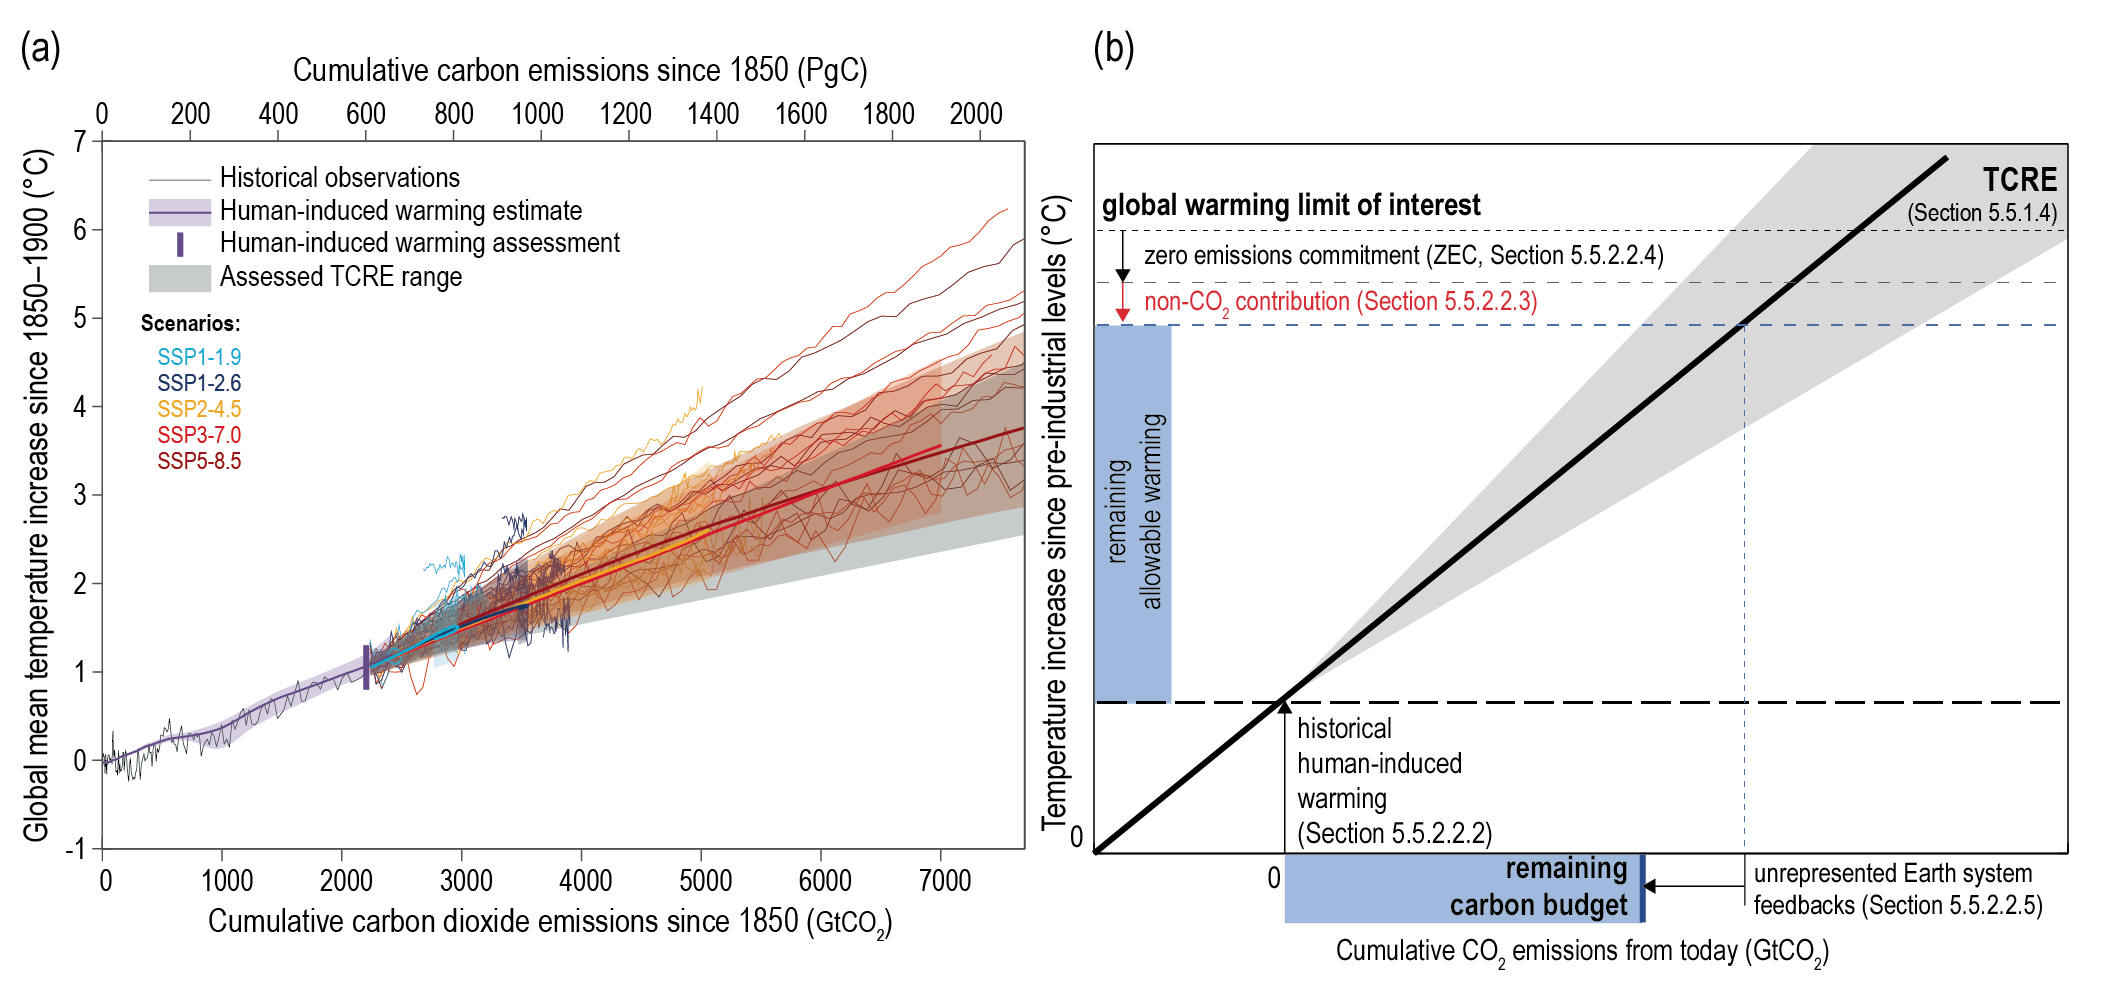
\includegraphics[width=\linewidth, totalheight=0.75\textheight, keepaspectratio]{future-IPCC_AR6_WGI_TS_Figure_18.png}
    \slidereference{IPCC AR6}
\end{frame}

\end{document}





% \begin{frame}{TITLE}
% \end{frame}